\documentclass[a4paper, 11pt]{report}
\usepackage[hidelinks]{hyperref}
\usepackage{amssymb}
\usepackage{amsmath}
\usepackage{amsthm}
\usepackage[utf8]{inputenc}
\usepackage[T1]{fontenc}
\usepackage{lmodern}
\usepackage{lipsum}
\usepackage[onehalfspacing]{setspace}
\usepackage[top=35mm, left=30mm, right=30mm]{geometry}
\usepackage{graphicx}
\usepackage{svg}
\usepackage{nameref}
\usepackage{graphicx}
\usepackage{xcolor}
\usepackage{colortbl}
\usepackage{subcaption}
\usepackage{cleveref}
\usepackage{tikz}
\usepackage{float}
\usepackage{listings}
\usepackage{extarrows}
\usepackage[main=ngerman]{babel}
\usepackage{marvosym}
\usepackage[nottoc]{tocbibind}
\hypersetup{hypertexnames=false}

\lstset{numbers=left, numberstyle=\tiny, numbersep=5pt}
\lstset{language=Python}

\usetikzlibrary{matrix}

\DeclareMathOperator{\rel}{\sim_R}
\renewcommand{\emph}[1]{\textit{#1}}
\newcommand{\mytitle}[1]{\LARGE{#1}\normalsize}
\newcommand{\titlespace}{\vspace{2.5em}}
\newcommand{\smallspace}{\vspace{1em}}
\newcommand{\hugespace}{\vspace{22em}}

\theoremstyle{definition}
\newtheorem{definition}{Definition}[section]
\newtheorem{example}[definition]{Beispiel}
\newtheorem{theorem}[definition]{Satz}
\newtheorem{corollary}[definition]{Korollar}
\newtheorem*{remark}{Bemerkung}
\newenvironment{myAbstract}{\section*{Abstract}}{}

\begin{document}
\pagenumbering{roman}
\newgeometry{top=35mm, left=25mm, right=25mm, bottom=10mm}
\begin{titlepage}
	\begin{center}
		\begin{minipage}{.49\textwidth}
			\flushleft
			\includesvg[width=\textwidth]{assets/uni-logo}
		\end{minipage}
		\begin{minipage}{.49\textwidth}
			\flushright
			\today\\
			\phantom{1}
		\end{minipage}
		\begin{minipage}{.49\textwidth}
			\begin{center}
				\vspace{2cm}
				Bachelorarbeit im Studiengang\\
				\glqq Angewandte Informatik\grqq{}\\
				\titlespace
				\mytitle{SUSAN}\\
				Ein Ansatz zur Strukturerkennung in Bildern\\
				\hugespace
				Institut für\\Numerische und Angewandte Mathematik\\
				\titlespace
				Bachelor und Masterarbeiten des Zentrums für angewandte Informatik an der Georg-August-Universität Göttingen\\
				\titlespace
				Julian Lüken\\
				\texttt{julian.lueken@stud.uni-goettingen.de}\\
			\end{center}
		\end{minipage}
	\end{center}
\end{titlepage}

\restoregeometry
\newgeometry{left=45mm, right=45mm}
\pagestyle{empty}
\setcounter{page}{2}

\pagebreak
\newgeometry{top=210mm}
\noindent
\begin{tabular}{l}
Georg-August-Universität Göttingen\\
Institut für Informatik\\
\end{tabular}\\[1em]
\begin{tabular}{ll}
	\Telefon 	&+49 (551) 39-172000\\
	\FAX 		&+49 (551) 39-14403\\
	\Letter 	&\texttt{office@informatik.uni-goettingen.de}\\
\end{tabular}\\[1em]
\begin{tabular}{l}
\texttt{www.informatik.uni-goettingen.de}\\
\end{tabular}\\[1em]

\pagebreak

\noindent Ich erkläre hiermit, dass ich die vorliegende Arbeit selbständig verfasst und keine anderen als die angegebenen Quellen und Hilfsmittel verwendet habe.\\[0.7em]
\phantom{H}
\includegraphics[height=3em]{sign.png}\\[0.5em]
Göttingen, den \today \hspace{2em}

\pagebreak
\restoregeometry
\pagenumbering{arabic}
\setcounter{page}{0}
\newgeometry{left=45mm, right=45mm}
\tableofcontents

\pagebreak

\restoregeometry

\pagestyle{headings}

\chapter{Einführung}
	Ein Kantendetektor ist ein Werkzeug, welches die Stellen der größten Intensitätsunterschiede in Digitalbildern feststellt und markiert. Der Mensch kann durch sein Sehvermögen mit Leichtigkeit Kanten lokalisieren. Um diesen Prozess zu automatisieren, benötigen wir allerdings ein mathematisches Prinzip, welches unabhängig vom spezifischen Bild pixelgenaue Resultate liefert.

	Auf der Kantendetektion basieren viele weiterführende Verfahren, zum Beispiel aus den Feldern der kantenbasierten Bildverbesserung und des maschinellen Sehens, in denen die für das menschliche Auge wichtige optische Information über die Position, Länge und Orientierung der Kanten auf den jeweiligen digitalen Bildern in besonderem Maße berücksichtigt wird.

	Ein solcher Kantendetektor, nämlich der \emph{SUSAN}-Kantendetektor (\emph{smallest univalue segment assimilating nucleus}) aus \cite{SUSAN}, wird in dieser Arbeit im Detail vorgestellt. Die zugrundeliegende Idee ist, für jeden Punkt des Bildes festzustellen, welcher Anteil einer diesen Punkt umgebenden Fläche des Bildes \glqq ähnlich\grqq{} zu dem Punkt ist. Dabei meint \glqq Ähnlichkeit\grqq{} in diesem Fall, dass der Intensitätsunterschied unter einer vorgegebenen Grenze liegt. Jede einem Punkt zugehörige Fläche ähnlicher Punkte nennen wir \emph{USAN} (\emph{univalue segment assimilating nucleus}). Unser Ziel ist es, die Punkte (oder Nuklei) der kleinsten USANs zu markieren. Zusätzlich habe ich den \emph{SUSAN}-Kantendetektor in Python 3 implementiert (\cite{mysoftware}).

	Im ersten Kapitel dieser Arbeit besprechen wir die mathematischen Grundlagen der Bildverarbeitung. Im zweiten Kapitel wird der Kantendetektor neben meiner persönlichen Implementation des Kantendetektors vorgestellt und mit dem Kantendetektor von Canny verglichen. Zuletzt diskutiere ich die Vor- und Nachteile des \emph{SUSAN}-Kantendetektors und meiner Implementation. Der SUSAN-Kantendetektor basiert auf einem ähnlichen Prinzip: Anhand der Umgebung eines jeden Pixels wird entschieden, ob ein Teil einer Kante vorliegt oder nicht.

\chapter{Mathematische Grundlagen}
	\section{Bildverarbeitung}\label{sec:imageproc}
		In der digitalen Bildverarbeitung für Graustufenbilder betrachten wir Abbildungen der Form
		$$ I: [0, B-1]_\mathbb{Z} \times [0, H-1]_\mathbb{Z} \to [0,255]_\mathbb{Z}. $$
		$H$ steht für die Höhe und $B$ für die Breite des Bildes. Ferner steht $0$ für schwarz und $255$ für weiß. Solche Abbildungen werden im weiteren Verlauf dieser Arbeit schlichtweg als Bilder bezeichnet.

		Eines der wichtigen Instrumente der Bildverarbeitung ist die Faltung. Die Faltung ist für Funktionen $f,g : \mathbb{R}^k \to \mathbb{R}$ definiert als
		$$ (f * g)(x) = \int_{\mathbb{R}^k} f(s) \; ds.$$
		Für $k = 2$ und $(x,y) \in \mathbb{R}^2$ bedeutet diese Definition insbesondere
		$$ (f*g)(x, y) = \int_{-\infty}^{\infty} \int_{-\infty}^{\infty} f(s, t) \; g(x - s, y - t) \; ds \; dt.$$

		Digitale Bilder liegen zwar in der Praxis zweidimensional vor, allerdings nur diskret; passend zur Definition von $I$. Für den diskreten Fall mit endlichen Grenzen benötigen wir nun also einen diskreten Faltungsoperator. Dieser Operator trägt den Namen \emph{Filtermaske}.
		Eine Filtermaske ist eine Matrix $K \in \mathbb{R}^{n \times m}$, die folgendermaßen Anwendung findet:
		
		$$ O(x,y) = \sum_{i=0}^{n-1} \sum_{j=0}^{m-1} K(i,j) \cdot I(x-i+a, y-j+b),$$
		
		für $(x,y) \in [0, B-1]_\mathbb{Z} \times [0, H-1]_\mathbb{Z}$, wobei $(a,b)$ der Nukleus der Filtermaske ist, $I$ das Eingangsbild und $O$ das neu gewonnene Ausgangsbild. Außerhalb des Definitionsbereichs von $I$ sei für diese Definition $I \equiv 0$.
		Wir schreiben, wie bei der Faltung
		$$ O = K * I.$$

		Ein Beispiel für eine solche Filtermaske bietet der sogenannte Gaußsche Weichzeichner, der in \cite{gaussianblur} näher beschrieben wird. Im stetigen Fall wendet man ihn an, indem man eine Eingangsfunktion mit der Normalverteilungsfunktion in zwei Dimensionen faltet. Die Funktion der Normalverteilung lautet für einen Parameter $\sigma > 0$:
		$$ g_\sigma(x,y) := \frac{1}{2 \pi \sigma} \;e ^{-\frac{x^2 + y^2}{2\sigma^2}}. $$
		Bevor wir mit einem diskreten Bild falten können, müssen wir eine endlich große, diskrete Filtermaske aus der Definition von $g$ gewinnen. Durch die Integration der Funktion um jedes Pixel erhalten wir
		$$\hat G_\sigma(x,y) = \int_{y-\frac{1}{2}}^{y+\frac{1}{2}} \int_{x-\frac{1}{2}}^{x+\frac{1}{2}} g_\sigma(s,t) \; ds \; dt.$$
		Für eine Anzahl $N$ an Stichproben können wir diese Integration durch Rechtecke approximieren.
		Man wähle eine Größe $n = m$ der Filtermaske und summiere für $x,y \in [-n, n]_\mathbb{Z}$ jeweils
		$$G_\sigma(x,y) = \frac{1}{N}\sum_{i=-\lceil\frac{N-1}{2}\rceil}^{\lfloor\frac{N-1}{2}\rfloor}\, \sum_{j=-\lceil\frac{N-1}{2}\rceil}^{\lfloor\frac{N-1}{2}\rfloor} g_\sigma(x+\frac{i}{N},y+\frac{j}{N})$$
		für ein passendes $\sigma$ und ein großes $N$.
		Die Größe der Filtermaske bestimmt sich in diesem Fall über das gewählte $\sigma$. Eine Faustregel dafür lautet, dass falls $\sqrt{\hat x^2 + \hat y^2} \geq 3\sigma$ gilt, auch $g(\hat x,\hat y) \approx 0$ gilt. Ausgehend davon können wir $n = \lfloor3\sigma\rfloor-1$ wählen und erhalten somit die Filtermaske
		$$G = \frac{1}{273}
		\begin{pmatrix}
			1&4&7&4&1\\
			4&16&26&16&4\\
			7&26&41&26&7\\
			4&16&26&16&4\\
			1&4&7&4&1
		\end{pmatrix}$$
 		für $\sigma = 1$, $N = 1000$ und $n = 2$. Wenden wir nun unseren Operator $G$ auf das folgende linke Bild an, so erhalten wir das nachstehende rechte Bild aus Abbildung \ref{fig:gaussian-example}:
		\begin{center}
			\begin{figure}[H]
				\begin{minipage}{.475\textwidth} \centering \small
					\begin{tikzpicture}[fill=black, text=white]
						\matrix(m)[matrix of nodes, nodes={draw, minimum size = .9cm}, column sep=-\pgflinewidth,row sep=-\pgflinewidth]{
							|[fill]|0	&|[fill]|0	&|[fill]|0	&|[text=black, fill=white]|255	&|[fill]|0	&|[fill]|0	&|[fill]|0\\
							|[fill]|0	&|[fill]|0	&|[fill]|0	&|[text=black, fill=white]|255	&|[fill]|0	&|[fill]|0	&|[fill]|0\\
							|[fill]|0	&|[fill]|0	&|[fill]|0	&|[text=black, fill=white]|255	&|[fill]|0	&|[fill]|0	&|[fill]|0\\
							|[fill]|0	&|[fill]|0	&|[fill]|0	&|[text=black, fill=white]|255	&|[fill]|0	&|[fill]|0	&|[fill]|0\\
							|[fill]|0	&|[fill]|0	&|[fill]|0	&|[text=black, fill=white]|255	&|[fill]|0	&|[fill]|0	&|[fill]|0\\
							|[fill]|0	&|[fill]|0	&|[fill]|0	&|[text=black, fill=white]|255	&|[fill]|0	&|[fill]|0	&|[fill]|0\\
							|[fill]|0	&|[fill]|0	&|[fill]|0	&|[text=black, fill=white]|255	&|[fill]|0	&|[fill]|0	&|[fill]|0\\
						};
					\end{tikzpicture}
				\end{minipage}
				\begin{minipage}{.05\textwidth}
					\centering \normalsize $\xlongrightarrow{G*}$
				\end{minipage}
				\begin{minipage}{.475\textwidth} \centering \small
					\begin{tikzpicture}[fill=black, text=white]
						\matrix(m)[matrix of nodes, nodes={draw, minimum size = .9cm}, column sep=-\pgflinewidth,row sep=-\pgflinewidth]{
							|[fill=white!0!black]|0	&|[fill=white!4!black]|11	&|[fill=white!16!black]|43	&|[fill=white!27!black]|69	&|[fill=white!16!black]|43	&|[fill=white!4!black]|11	&|[fill=white!0!black]|0	\\ 
							|[fill=white!0!black]|0	&|[fill=white!5!black]|15	&|[fill=white!22!black]|58	&|[fill=white!36!black]|93	&|[fill=white!22!black]|58	&|[fill=white!5!black]|15	&|[fill=white!0!black]|0	\\ 
							|[fill=white!0!black]|0	&|[fill=white!6!black]|16	&|[fill=white!24!black]|62	&|[fill=white!39!black]|100	&|[fill=white!24!black]|62	&|[fill=white!6!black]|16	&|[fill=white!0!black]|0	\\ 
							|[fill=white!0!black]|0	&|[fill=white!6!black]|16	&|[fill=white!24!black]|62	&|[fill=white!39!black]|100	&|[fill=white!24!black]|62	&|[fill=white!6!black]|16	&|[fill=white!0!black]|0	\\ 
							|[fill=white!0!black]|0	&|[fill=white!6!black]|16	&|[fill=white!24!black]|62	&|[fill=white!39!black]|100	&|[fill=white!24!black]|62	&|[fill=white!6!black]|16	&|[fill=white!0!black]|0	\\ 
							|[fill=white!0!black]|0	&|[fill=white!5!black]|15	&|[fill=white!22!black]|58	&|[fill=white!36!black]|93	&|[fill=white!22!black]|58	&|[fill=white!5!black]|15	&|[fill=white!0!black]|0	\\ 
							|[fill=white!0!black]|0	&|[fill=white!4!black]|11	&|[fill=white!16!black]|43	&|[fill=white!27!black]|69	&|[fill=white!16!black]|43	&|[fill=white!4!black]|11	&|[fill=white!0!black]|0	\\ 
						};
					\end{tikzpicture}
				\end{minipage}
			\normalsize
			\caption{Die berechnete Gauß-Filtermaske in Aktion.}
			\label{fig:gaussian-example}
			\end{figure}
		\end{center}

		Dadurch, dass wir das Eingangsbild $I$ außerhalb des Randes 0 setzen, erhalten wir keinerlei Artefakte am Rand. Als Rechenbeispiel benutzen wir jetzt das mittlere Pixel $(x,y) = (3,3)$ aus Abbildung \ref{fig:gaussian-example}:

		\begin{align*}
			O(3,3) 	&= \sum_{i=0}^{4} \sum_{j=0}^{4} G(i,j) \cdot I(3-i+2, 3-j+2) 											\\
					&= \sum_{i=0}^{4} \sum_{j=0}^{4} G(i,j) \cdot I(5-i, 5-j) 												\\
					&= \frac{1}{273} \left( 255 \cdot 7 + 255 \cdot 26 + 255 \cdot 41 + 255 \cdot 26 + 255 \cdot 7 \right) 	\\
					&= \frac{255}{273} \left(7 + 26 + 41 + 26 + 7 \right) = 99.94 \approx 100.
		\end{align*}

		In der Praxis dient der Gaußsche Weichzeichner dem Glätten von Bildern. Dadurch können kleine Artefakte aus Digitalbildern entfernt werden. In einigen Verfahren, wie zum Beispiel dem Kantedetektor von Canny aus \cite{canny}, wird der Gaußsche Weichzeichner zu diesem Zwecke verwendet.

\chapter{Der SUSAN Kantendetektor}
	In diesem Kapitel stellen wir den Kantendetektions-Algorithmus nach dem SUSAN Prinzip aus \cite{SUSAN} vor. Danach erläutern wir einige Details zur Implementation des Algorithmus in Python 3. Im dritten Abschnitt vergleichen wir den SUSAN-Kantendetektor mit dem Kantendetektor von Canny und im letzten Abschnitt leiten wir her, warum der SUSAN-Kantendetektor funktioniert.

	\section{Der Algorithmus}\label{sec:thealgorithm}
		Der SUSAN Kantendetektor aus \cite{SUSAN} besteht aus drei Großschritten:

		Im ersten Schritt, den wir in Abschnitt \ref{ssec:susan_principle} besprechen, legen wir eine Maske über jedes Pixel. Mithilfe dieser Maske berechnen wir für jedes Pixel eine Kennzahl $A$, die im weiteren Verlauf dieser Arbeit \glqq Antwort\grqq{} heißt. Die lokalen Maxima von $A$ liegen genau auf den lokalen Extrema der partiellen Ableitungen in horizontaler und vertikaler Richtung unseres Eingangsbildes $I$, wie wir später noch zeigen.

		Der zweite Schritt in Abschnitt \ref{ssec:nonmax} ist die sogenannte Non-Maximum-Suppression, bei der wir mithilfe der Richtung der im ersten Schritt berechneten Antwort die Kanten im Eingangsbild $I$ noch genauer lokalisieren, indem wir nur Züge der Kanten erhalten, deren Antwort lokal maximal ist.

		Falsch positive und falsch negative Ergebnisse sind auf mit Rauschen behafteten Digitalbildern keine Seltenheit. Aus diesem Grund gibt es noch einen dritten Ausdünnungsschritt, in welchem bei Bedarf räumlich isolierte Antworten entfernt werden und Kanten vervollständigt werden. Diesen Schritt behandeln wir näher im Abschnitt \ref{ssec:thinout}.

		Anschließend wird im letzten Teil dieses Kapitels, Abschnitt \ref{ssec:corner_detector}, der Eckendetektor des SUSAN-Prinzips vorgestellt. Durch kleine Änderungen an den ersten zwei Schritten können so, zusätzlich zu Kanten, ebenfalls Ecken gefunden werden.

		\subsection{Das USAN-Prinzip}\label{ssec:susan_principle}
			Sei $I: [0, B-1]_\mathbb{Z} \times [0, H-1]_\mathbb{Z} \to [0,255]_\mathbb{Z}$ ein Eingangsbild. Um jedes Pixel im Bild legen wir eine Maske. Für unseren Zweck betrachten wir lediglich die Masken der Größe $3\times3$ beziehungsweise $7\times7$, wie sie in Abbildung \ref{fig:def_masken} dargestellt sind.
			\begin{figure}[H]
				\begin{center}
					\begin{tikzpicture}[fill=orange]
						\matrix(m)[matrix of nodes, nodes={draw, minimum size = 0.5cm}, nodes in empty cells, column sep=-\pgflinewidth,row sep=-\pgflinewidth]{
									&			&			&			&			&			&			\\
									&			&			&			&			&			&			\\
									&			&|[fill]|	&|[fill]|	&|[fill]|	&			&			\\
									&			&|[fill]|	&|[fill=yellow]|	&|[fill]|	&			&			\\
									&			&|[fill]|	&|[fill]|	&|[fill]|	&			&			\\
									&			&			&			&			&			&			\\
									&			&			&			&			&			&			\\
						};
					\end{tikzpicture}\qquad
					\begin{tikzpicture}[fill=orange]
						\matrix(m)[matrix of nodes, nodes={draw, minimum size = 0.5cm}, nodes in empty cells, column sep=-\pgflinewidth,row sep=-\pgflinewidth]{
									&			&|[fill]|	&|[fill]|	&|[fill]|	&			&			\\
									&|[fill]|	&|[fill]|	&|[fill]|	&|[fill]|	&|[fill]|	&			\\
						|[fill]|	&|[fill]|	&|[fill]|	&|[fill]|	&|[fill]|	&|[fill]|	&|[fill]|	\\
						|[fill]|	&|[fill]|	&|[fill]|	&|[fill=yellow]|	&|[fill]|	&|[fill]|	&|[fill]|	\\
						|[fill]|	&|[fill]|	&|[fill]|	&|[fill]|	&|[fill]|	&|[fill]|	&|[fill]|	\\
									&|[fill]|	&|[fill]|	&|[fill]|	&|[fill]|	&|[fill]|	&			\\
									&			&|[fill]|	&|[fill]|	&|[fill]|	&			&			\\
						};
					\end{tikzpicture}
					\caption{Die zwei Filtermaskenträger. Links $3\times3$, rechts $7\times7$. Dabei ist das gelbe Pixel der Mittelpunkt oder Nukleus der Maske, die orangenen Pixel liegen in der Maske und die weißen Pixel außerhalb der Maske.}
					\label{fig:def_masken}
				\end{center}
			\end{figure}
			
			Die Maskenträger sind Umgebungen eines Pixels, die einen Kreis approximieren. Der $3 \times 3$ Maskenträger approximiert einen Kreis mit einem Radius von $1,4$ Pixeln, der $7 \times 7$ Maskenträger hingegen approximiert einen Kreis mit einem Radius von $3,4$ Pixeln.

			Prinzipiell finden wir beim ersten Schritt des SUSAN-Verfahrens für jeden Nukleus $r_0 \in [0, B-1]_\mathbb{Z} \times [0, H-1]_\mathbb{Z}$ die Anzahl $n(r_0)$ der zu ihm ähnlichen Pixel im Maskenträger. Mit \glqq ähnlich\grqq{} ist in diesem Kontext gemeint, dass die absolute Intensitätsdifferenz $|I(r)-I(r_0)|$ zwischen den beiden Pixeln $r$ und $r_0$ unter einer im Vorfeld festgelegten Grenze $t \geq 1$ liegt, wobei $r$ ein Pixel aus dem Maskenträger ist. Die ähnlichen Pixel bezeichnen wir ferner als USAN (\emph{univalue segment assimilating nucleus}). Die maximale Größe einer USAN ist für die $7 \times 7$ Maske $36$ und für die $3 \times 3$ Maske $8$. $g$ ist der sogenannte geometrische Schwellenwert und wird gewählt als maximale Größe einer USAN. Um die Antwort $A(r_0)$ zu erhalten, subtrahieren wir die Anzahl $n(r_0)$ der ähnlichen Pixel von $g$.

			Konkret führen wir folgende Rechnung durch.
			Für jedes Pixel $r_0$ in $I$, wobei $I(r_0)$ der Grauwert am Pixel $r_0$ ist, berechnen wir
				$$A(r_0) = \text{max}\{0, g - n(r_0)\}.$$
			Dabei ist $n$ definiert als
				$$n(r_0) = \sum_r c_t(r, r_0),$$
			wobei wir über alle Pixel $r$ in der Maske und $r_0$ selbst summieren und
				$$
					c_t(r, r_0) =
						\begin{cases}
							1 	& \text{falls } |I(r) - I(r_0)| \leq t, 	\\
							0 	& \text{sonst}
						\end{cases}
				$$
			eine Vergleichsfunktion für zwei Pixel ist. In der USAN von $r_0$ liegen genau diejenigen Pixel $r$ aus der Maske, für die $c_t(r, r_0) > 0$ gilt. Wir verbleiben mit der Antwort $A$, in welcher wir schon sehr gut den Effekt der Kantendetektion beobachten können.

			\begin{figure}[H]
				\centering
				\begin{tikzpicture}[fill=black, text=white]
					\tiny
					\matrix(m)[matrix of nodes, nodes={draw, minimum size = .6cm}, column sep=-\pgflinewidth,row sep=-\pgflinewidth]{
						|[fill=white!100!black, text=black]|255	&|[fill=white!100!black, text=black]|255	&|[fill=white!100!black, text=black]|255	&|[fill=white!100!black, text=black]|255	&|[fill=white!100!black, text=black]|255	&|[fill=white!0!black]|0	&|[fill=white!100!black, text=black]|255	&|[fill=white!100!black, text=black]|255	&|[fill=white!100!black, text=black]|255	&|[fill=white!100!black, text=black]|255	&|[fill=white!100!black, text=black]|255	\\ 
						|[fill=white!100!black, text=black]|255	&|[fill=white!100!black, text=black]|255	&|[fill=white!100!black, text=black]|255	&|[fill=white!100!black, text=black]|255	&|[fill=white!100!black, text=black]|255	&|[fill=white!0!black]|0	&|[fill=white!100!black, text=black]|255	&|[fill=white!100!black, text=black]|255	&|[fill=white!100!black, text=black]|255	&|[fill=white!100!black, text=black]|255	&|[fill=white!100!black, text=black]|255	\\ 
						|[fill=white!100!black, text=black]|255	&|[fill=white!100!black, text=black]|255	&|[fill=white!100!black, text=black]|255	&|[fill=white!100!black, text=black]|255	&|[fill=white!100!black, text=black]|255	&|[fill=white!0!black]|0	&|[fill=white!100!black, text=black]|255	&|[fill=white!100!black, text=black]|255	&|[fill=white!100!black, text=black]|255	&|[fill=white!100!black, text=black]|255	&|[fill=white!100!black, text=black]|255	\\ 
						|[fill=white!100!black, text=black]|255	&|[fill=white!100!black, text=black]|255	&|[fill=white!100!black, text=black]|255	&|[fill=white!100!black, text=black]|255	&|[fill=white!100!black, text=black]|255	&|[fill=white!0!black]|0	&|[fill=white!100!black, text=black]|255	&|[fill=white!100!black, text=black]|255	&|[fill=white!100!black, text=black]|255	&|[fill=white!100!black, text=black]|255	&|[fill=white!100!black, text=black]|255	\\ 
						|[fill=white!100!black, text=black]|255	&|[fill=white!100!black, text=black]|255	&|[fill=white!100!black, text=black]|255	&|[fill=white!100!black, text=black]|255	&|[fill=white!100!black, text=black]|255	&|[fill=white!0!black]|0	&|[fill=white!100!black, text=black]|255	&|[fill=white!100!black, text=black]|255	&|[fill=white!100!black, text=black]|255	&|[fill=white!100!black, text=black]|255	&|[fill=white!100!black, text=black]|255	\\ 
						|[fill=white!100!black, text=black]|255	&|[fill=white!100!black, text=black]|255	&|[fill=white!100!black, text=black]|255	&|[fill=white!100!black, text=black]|255	&|[fill=white!100!black, text=black]|255	&|[fill=white!0!black]|0	&|[fill=white!100!black, text=black]|255	&|[fill=white!100!black, text=black]|255	&|[fill=white!100!black, text=black]|255	&|[fill=white!100!black, text=black]|255	&|[fill=white!100!black, text=black]|255	\\ 
						|[fill=white!100!black, text=black]|255	&|[fill=white!100!black, text=black]|255	&|[fill=white!100!black, text=black]|255	&|[fill=white!100!black, text=black]|255	&|[fill=white!100!black, text=black]|255	&|[fill=white!0!black]|0	&|[fill=white!100!black, text=black]|255	&|[fill=white!100!black, text=black]|255	&|[fill=white!100!black, text=black]|255	&|[fill=white!100!black, text=black]|255	&|[fill=white!100!black, text=black]|255	\\ 
						|[fill=white!100!black, text=black]|255	&|[fill=white!100!black, text=black]|255	&|[fill=white!100!black, text=black]|255	&|[fill=white!100!black, text=black]|255	&|[fill=white!100!black, text=black]|255	&|[fill=white!0!black]|0	&|[fill=white!100!black, text=black]|255	&|[fill=white!100!black, text=black]|255	&|[fill=white!100!black, text=black]|255	&|[fill=white!100!black, text=black]|255	&|[fill=white!100!black, text=black]|255	\\ 
						|[fill=white!100!black, text=black]|255	&|[fill=white!100!black, text=black]|255	&|[fill=white!100!black, text=black]|255	&|[fill=white!100!black, text=black]|255	&|[fill=white!100!black, text=black]|255	&|[fill=white!0!black]|0	&|[fill=white!100!black, text=black]|255	&|[fill=white!100!black, text=black]|255	&|[fill=white!100!black, text=black]|255	&|[fill=white!100!black, text=black]|255	&|[fill=white!100!black, text=black]|255	\\ 
						|[fill=white!100!black, text=black]|255	&|[fill=white!100!black, text=black]|255	&|[fill=white!100!black, text=black]|255	&|[fill=white!100!black, text=black]|255	&|[fill=white!100!black, text=black]|255	&|[fill=white!0!black]|0	&|[fill=white!100!black, text=black]|255	&|[fill=white!100!black, text=black]|255	&|[fill=white!100!black, text=black]|255	&|[fill=white!100!black, text=black]|255	&|[fill=white!100!black, text=black]|255	\\ 
						|[fill=white!100!black, text=black]|255	&|[fill=white!100!black, text=black]|255	&|[fill=white!100!black, text=black]|255	&|[fill=white!100!black, text=black]|255	&|[fill=white!100!black, text=black]|255	&|[fill=white!0!black]|0	&|[fill=white!100!black, text=black]|255	&|[fill=white!100!black, text=black]|255	&|[fill=white!100!black, text=black]|255	&|[fill=white!100!black, text=black]|255	&|[fill=white!100!black, text=black]|255	\\ 
					};
					\normalsize
				\end{tikzpicture}
				\begin{tikzpicture}[fill=black, text=white]
					\tiny
					\matrix(m)[matrix of nodes, nodes={draw, minimum size = .6cm}, column sep=-\pgflinewidth,row sep=-\pgflinewidth]{
						|[fill=white!66!black, text=black]|170	&|[fill=white!33!black]|85	&|[fill=white!33!black]|85	&|[fill=white!33!black]|85	&|[fill=white!66!black, text=black]|170	&|[fill=white!100!black, text=black]|255	&|[fill=white!66!black, text=black]|170	&|[fill=white!33!black]|85	&|[fill=white!33!black]|85	&|[fill=white!33!black]|85	&|[fill=white!66!black, text=black]|170	\\ 
						|[fill=white!33!black]|85	&|[fill=white!0!black]|0	&|[fill=white!0!black]|0	&|[fill=white!0!black]|0	&|[fill=white!33!black]|85	&|[fill=white!83!black, text=black]|212	&|[fill=white!33!black]|85	&|[fill=white!0!black]|0	&|[fill=white!0!black]|0	&|[fill=white!0!black]|0	&|[fill=white!33!black]|85	\\ 
						|[fill=white!33!black]|85	&|[fill=white!0!black]|0	&|[fill=white!0!black]|0	&|[fill=white!0!black]|0	&|[fill=white!33!black]|85	&|[fill=white!83!black, text=black]|212	&|[fill=white!33!black]|85	&|[fill=white!0!black]|0	&|[fill=white!0!black]|0	&|[fill=white!0!black]|0	&|[fill=white!33!black]|85	\\ 
						|[fill=white!33!black]|85	&|[fill=white!0!black]|0	&|[fill=white!0!black]|0	&|[fill=white!0!black]|0	&|[fill=white!33!black]|85	&|[fill=white!83!black, text=black]|212	&|[fill=white!33!black]|85	&|[fill=white!0!black]|0	&|[fill=white!0!black]|0	&|[fill=white!0!black]|0	&|[fill=white!33!black]|85	\\ 
						|[fill=white!33!black]|85	&|[fill=white!0!black]|0	&|[fill=white!0!black]|0	&|[fill=white!0!black]|0	&|[fill=white!33!black]|85	&|[fill=white!83!black, text=black]|212	&|[fill=white!33!black]|85	&|[fill=white!0!black]|0	&|[fill=white!0!black]|0	&|[fill=white!0!black]|0	&|[fill=white!33!black]|85	\\ 
						|[fill=white!33!black]|85	&|[fill=white!0!black]|0	&|[fill=white!0!black]|0	&|[fill=white!0!black]|0	&|[fill=white!33!black]|85	&|[fill=white!83!black, text=black]|212	&|[fill=white!33!black]|85	&|[fill=white!0!black]|0	&|[fill=white!0!black]|0	&|[fill=white!0!black]|0	&|[fill=white!33!black]|85	\\ 
						|[fill=white!33!black]|85	&|[fill=white!0!black]|0	&|[fill=white!0!black]|0	&|[fill=white!0!black]|0	&|[fill=white!33!black]|85	&|[fill=white!83!black, text=black]|212	&|[fill=white!33!black]|85	&|[fill=white!0!black]|0	&|[fill=white!0!black]|0	&|[fill=white!0!black]|0	&|[fill=white!33!black]|85	\\ 
						|[fill=white!33!black]|85	&|[fill=white!0!black]|0	&|[fill=white!0!black]|0	&|[fill=white!0!black]|0	&|[fill=white!33!black]|85	&|[fill=white!83!black, text=black]|212	&|[fill=white!33!black]|85	&|[fill=white!0!black]|0	&|[fill=white!0!black]|0	&|[fill=white!0!black]|0	&|[fill=white!33!black]|85	\\ 
						|[fill=white!33!black]|85	&|[fill=white!0!black]|0	&|[fill=white!0!black]|0	&|[fill=white!0!black]|0	&|[fill=white!33!black]|85	&|[fill=white!83!black, text=black]|212	&|[fill=white!33!black]|85	&|[fill=white!0!black]|0	&|[fill=white!0!black]|0	&|[fill=white!0!black]|0	&|[fill=white!33!black]|85	\\ 
						|[fill=white!33!black]|85	&|[fill=white!0!black]|0	&|[fill=white!0!black]|0	&|[fill=white!0!black]|0	&|[fill=white!33!black]|85	&|[fill=white!83!black, text=black]|212	&|[fill=white!33!black]|85	&|[fill=white!0!black]|0	&|[fill=white!0!black]|0	&|[fill=white!0!black]|0	&|[fill=white!33!black]|85	\\ 
						|[fill=white!66!black, text=black]|170	&|[fill=white!33!black]|85	&|[fill=white!33!black]|85	&|[fill=white!33!black]|85	&|[fill=white!66!black, text=black]|170	&|[fill=white!100!black, text=black]|255	&|[fill=white!66!black, text=black]|170	&|[fill=white!33!black]|85	&|[fill=white!33!black]|85	&|[fill=white!33!black]|85	&|[fill=white!66!black, text=black]|170	\\ 
					};
					\normalsize
				\end{tikzpicture}
				\caption{Das USAN Prinzip (links Eingang, rechts Antwort, $t=1$, $3\times3$ Maske).}
				\label{fig:susan_principle}
			\end{figure}

			Nehmen wir nun zum Beispiel ein Eingangsbild wie in Abbildung \ref{fig:susan_principle}. Hier wurde der oben genannte Algorithmus angewandt.
			Sehen wir uns das mittlere Pixel $a$ des Eingangsbilds an und wenden den Algorithmus mit $t=1$ an:
			\begin{align*}
				n(a) 	=&\sum_r c(r,a) \\
						=&\; 0 + 1 + 0 \\
						+&\; 0 + 1 + 0 \\
						+&\; 0 + 1 + 0 = 3,
			\end{align*}
			$$ A(a) = g - n(a) = 8 - 3 = 5. $$
			Um den Effekt hervorzuheben, wird jeder Graustufenwert mit der maximalen Antwort normiert und dann mit $255$, dem Maximalwert, der für die Farbe weiß steht, multipliziert. Jeder Graustufenwert wird also mit dem Faktor $\frac{255}{\max_{r_0}{A(r_0)}}$ multipliziert. In diesem Fall erreicht ein Pixel $b$ am Ende der Kante den Maximalwert, da
			\begin{align*}
				n(b) 	=&\sum_r c(r,b) \\
						=&\; 0 + 1 + 0 \\
						+&\; 0 + 1 + 0 = 2,
			\end{align*}
			$$ A(b) = g - n(b) = 8 - 2 = 6. $$
			Wir multiplizieren also in unserer Darstellung $A(b)$ mit $\frac{255}{6}$. Somit erhalten wir an der Stelle $a$ den Wert $212$ und an der Stelle $b$ den Wert $255$.
			Zunächst einmal finden wir, dass $A$ genau da am größten ist, wo unser Eingangsbild eine Kante hat. Es besteht noch das Problem, dass nicht nur auf Kanten, sondern bereits in der Nähe von Kanten $A > 0$ ist. Wir schließen daraus, dass die Lokalisation der Kanten zwar durchaus funktioniert, aber verbesserungswürdig ist.

			\begin{figure}[H]\centering
				\begin{tikzpicture}[fill=black, text=white]
					\tiny
					\matrix(m)[matrix of nodes, nodes={draw, minimum size = .6cm}, column sep=-\pgflinewidth,row sep=-\pgflinewidth]{
						|[fill=white!100!black, text=black]|255	&|[fill=white!100!black, text=black]|255	&|[fill=white!100!black, text=black]|255	&|[fill=white!100!black, text=black]|255	&|[fill=white!100!black, text=black]|255	&|[fill=white!100!black, text=black]|255	&|[fill=white!100!black, text=black]|255	&|[fill=white!100!black, text=black]|255	&|[fill=white!100!black, text=black]|255	&|[fill=white!100!black, text=black]|255	&|[fill=white!100!black, text=black]|255	\\ 
						|[fill=white!100!black, text=black]|255	&|[fill=white!100!black, text=black]|255	&|[fill=white!100!black, text=black]|255	&|[fill=white!100!black, text=black]|255	&|[fill=white!100!black, text=black]|255	&|[fill=white!100!black, text=black]|255	&|[fill=white!100!black, text=black]|255	&|[fill=white!100!black, text=black]|255	&|[fill=white!100!black, text=black]|255	&|[fill=white!100!black, text=black]|255	&|[fill=white!100!black, text=black]|255	\\ 
						|[fill=white!100!black, text=black]|255	&|[fill=white!100!black, text=black]|255	&|[fill=white!100!black, text=black]|255	&|[fill=white!100!black, text=black]|255	&|[fill=white!100!black, text=black]|255	&|[fill=white!100!black, text=black]|255	&|[fill=white!100!black, text=black]|255	&|[fill=white!100!black, text=black]|255	&|[fill=white!100!black, text=black]|255	&|[fill=white!100!black, text=black]|255	&|[fill=white!100!black, text=black]|255	\\ 
						|[fill=white!100!black, text=black]|255	&|[fill=white!100!black, text=black]|255	&|[fill=white!100!black, text=black]|255	&|[fill=white!0!black]|0	&|[fill=white!0!black]|0	&|[fill=white!0!black]|0	&|[fill=white!0!black]|0	&|[fill=white!0!black]|0	&|[fill=white!100!black, text=black]|255	&|[fill=white!100!black, text=black]|255	&|[fill=white!100!black, text=black]|255	\\ 
						|[fill=white!100!black, text=black]|255	&|[fill=white!100!black, text=black]|255	&|[fill=white!100!black, text=black]|255	&|[fill=white!0!black]|0	&|[fill=white!0!black]|0	&|[fill=white!0!black]|0	&|[fill=white!0!black]|0	&|[fill=white!0!black]|0	&|[fill=white!100!black, text=black]|255	&|[fill=white!100!black, text=black]|255	&|[fill=white!100!black, text=black]|255	\\ 
						|[fill=white!100!black, text=black]|255	&|[fill=white!100!black, text=black]|255	&|[fill=white!100!black, text=black]|255	&|[fill=white!0!black]|0	&|[fill=white!0!black]|0	&|[fill=white!0!black]|0	&|[fill=white!0!black]|0	&|[fill=white!0!black]|0	&|[fill=white!100!black, text=black]|255	&|[fill=white!100!black, text=black]|255	&|[fill=white!100!black, text=black]|255	\\ 
						|[fill=white!100!black, text=black]|255	&|[fill=white!100!black, text=black]|255	&|[fill=white!100!black, text=black]|255	&|[fill=white!0!black]|0	&|[fill=white!0!black]|0	&|[fill=white!0!black]|0	&|[fill=white!0!black]|0	&|[fill=white!0!black]|0	&|[fill=white!100!black, text=black]|255	&|[fill=white!100!black, text=black]|255	&|[fill=white!100!black, text=black]|255	\\ 
						|[fill=white!100!black, text=black]|255	&|[fill=white!100!black, text=black]|255	&|[fill=white!100!black, text=black]|255	&|[fill=white!0!black]|0	&|[fill=white!0!black]|0	&|[fill=white!0!black]|0	&|[fill=white!0!black]|0	&|[fill=white!0!black]|0	&|[fill=white!100!black, text=black]|255	&|[fill=white!100!black, text=black]|255	&|[fill=white!100!black, text=black]|255	\\ 
						|[fill=white!100!black, text=black]|255	&|[fill=white!100!black, text=black]|255	&|[fill=white!100!black, text=black]|255	&|[fill=white!100!black, text=black]|255	&|[fill=white!100!black, text=black]|255	&|[fill=white!100!black, text=black]|255	&|[fill=white!100!black, text=black]|255	&|[fill=white!100!black, text=black]|255	&|[fill=white!100!black, text=black]|255	&|[fill=white!100!black, text=black]|255	&|[fill=white!100!black, text=black]|255	\\ 
						|[fill=white!100!black, text=black]|255	&|[fill=white!100!black, text=black]|255	&|[fill=white!100!black, text=black]|255	&|[fill=white!100!black, text=black]|255	&|[fill=white!100!black, text=black]|255	&|[fill=white!100!black, text=black]|255	&|[fill=white!100!black, text=black]|255	&|[fill=white!100!black, text=black]|255	&|[fill=white!100!black, text=black]|255	&|[fill=white!100!black, text=black]|255	&|[fill=white!100!black, text=black]|255	\\ 
						|[fill=white!100!black, text=black]|255	&|[fill=white!100!black, text=black]|255	&|[fill=white!100!black, text=black]|255	&|[fill=white!100!black, text=black]|255	&|[fill=white!100!black, text=black]|255	&|[fill=white!100!black, text=black]|255	&|[fill=white!100!black, text=black]|255	&|[fill=white!100!black, text=black]|255	&|[fill=white!100!black, text=black]|255	&|[fill=white!100!black, text=black]|255	&|[fill=white!100!black, text=black]|255	\\ 
					};
					\normalsize
				\end{tikzpicture}
				\begin{tikzpicture}[fill=black, text=white]
					\tiny
					\matrix(m)[matrix of nodes, nodes={draw, minimum size = .6cm}, column sep=-\pgflinewidth,row sep=-\pgflinewidth]{
						|[fill=white!100!black, text=black]|255	&|[fill=white!49!black]|127	&|[fill=white!49!black]|127	&|[fill=white!49!black]|127	&|[fill=white!49!black]|127	&|[fill=white!49!black]|127	&|[fill=white!49!black]|127	&|[fill=white!49!black]|127	&|[fill=white!49!black]|127	&|[fill=white!49!black]|127	&|[fill=white!100!black, text=black]|255\\ 
						|[fill=white!49!black]|127	&|[fill=white!0!black]|0	&|[fill=white!0!black]|0	&|[fill=white!0!black]|0	&|[fill=white!0!black]|0	&|[fill=white!0!black]|0&|[fill=white!0!black]|0	&|[fill=white!0!black]|0	&|[fill=white!0!black]|0	&|[fill=white!0!black]|0	&|[fill=white!49!black]|127	\\ 
						|[fill=white!49!black]|127	&|[fill=white!0!black]|0	&|[fill=white!0!black]|0	&|[fill=white!24!black]|63	&|[fill=white!49!black]|127	&|[fill=white!49!black]|127	&|[fill=white!49!black]|127	&|[fill=white!24!black]|63	&|[fill=white!0!black]|0	&|[fill=white!0!black]|0	&|[fill=white!49!black]|127	\\ 
						|[fill=white!49!black]|127	&|[fill=white!0!black]|0	&|[fill=white!24!black]|63	&|[fill=white!100!black, text=black]|255	&|[fill=white!49!black]|127	&|[fill=white!49!black]|127	&|[fill=white!49!black]|127	&|[fill=white!100!black, text=black]|255	&|[fill=white!24!black]|63	&|[fill=white!0!black]|0	&|[fill=white!49!black]|127	\\ 
						|[fill=white!49!black]|127	&|[fill=white!0!black]|0	&|[fill=white!49!black]|127	&|[fill=white!49!black]|127	&|[fill=white!0!black]|0	&|[fill=white!0!black]|0&|[fill=white!0!black]|0	&|[fill=white!49!black]|127	&|[fill=white!49!black]|127	&|[fill=white!0!black]|0	&|[fill=white!49!black]|127	\\ 
						|[fill=white!49!black]|127	&|[fill=white!0!black]|0	&|[fill=white!49!black]|127	&|[fill=white!49!black]|127	&|[fill=white!0!black]|0	&|[fill=white!0!black]|0&|[fill=white!0!black]|0	&|[fill=white!49!black]|127	&|[fill=white!49!black]|127	&|[fill=white!0!black]|0	&|[fill=white!49!black]|127	\\ 
						|[fill=white!49!black]|127	&|[fill=white!0!black]|0	&|[fill=white!49!black]|127	&|[fill=white!49!black]|127	&|[fill=white!0!black]|0	&|[fill=white!0!black]|0&|[fill=white!0!black]|0	&|[fill=white!49!black]|127	&|[fill=white!49!black]|127	&|[fill=white!0!black]|0	&|[fill=white!49!black]|127	\\ 
						|[fill=white!49!black]|127	&|[fill=white!0!black]|0	&|[fill=white!24!black]|63	&|[fill=white!100!black, text=black]|255	&|[fill=white!49!black]|127	&|[fill=white!49!black]|127	&|[fill=white!49!black]|127	&|[fill=white!100!black, text=black]|255	&|[fill=white!24!black]|63	&|[fill=white!0!black]|0	&|[fill=white!49!black]|127	\\ 
						|[fill=white!49!black]|127	&|[fill=white!0!black]|0	&|[fill=white!0!black]|0	&|[fill=white!24!black]|63	&|[fill=white!49!black]|127	&|[fill=white!49!black]|127	&|[fill=white!49!black]|127	&|[fill=white!24!black]|63	&|[fill=white!0!black]|0	&|[fill=white!0!black]|0	&|[fill=white!49!black]|127	\\ 
						|[fill=white!49!black]|127	&|[fill=white!0!black]|0	&|[fill=white!0!black]|0	&|[fill=white!0!black]|0	&|[fill=white!0!black]|0	&|[fill=white!0!black]|0&|[fill=white!0!black]|0	&|[fill=white!0!black]|0	&|[fill=white!0!black]|0	&|[fill=white!0!black]|0	&|[fill=white!49!black]|127	\\ 
						|[fill=white!100!black, text=black]|255	&|[fill=white!49!black]|127	&|[fill=white!49!black]|127	&|[fill=white!49!black]|127	&|[fill=white!49!black]|127	&|[fill=white!49!black]|127	&|[fill=white!49!black]|127	&|[fill=white!49!black]|127	&|[fill=white!49!black]|127	&|[fill=white!49!black]|127	&|[fill=white!100!black, text=black]|255\\ 
					};
					\normalsize
				\end{tikzpicture}
				\caption{Das USAN Prinzip findet Ecken und hebt diese sogar in der Antwort hervor ($t=1$, $3\times3$ Maske).}
				\label{fig:susan_principle_corners}
			\end{figure}

			Am Beispiel in Abbildung \ref{fig:susan_principle_corners} können wir beobachten, dass das USAN-Prinzip Ecken besonders hervorhebt. Dieser Effekt spielt eine große Rolle im SUSAN-Eckendetektor, auf den im Abschnitt \ref{ssec:corner_detector} dieser Arbeit weiter eingegangen wird.

			\begin{figure}[H]\centering
				\begin{tikzpicture}[fill=black, text=white]
					\tiny
					\matrix(m)[matrix of nodes, nodes={draw, minimum size = .6cm}, column sep=-\pgflinewidth,row sep=-\pgflinewidth]{
						|[fill=white!0!black]|0	&|[fill=white!0!black]|0	&|[fill=white!0!black]|0	&|[fill=white!0!black]|0	&|[fill=white!40!black]|102	&|[fill=white!100!black, text=black]|255	&|[fill=white!40!black]|102	&|[fill=white!0!black]|0	&|[fill=white!0!black]|0	&|[fill=white!0!black]|0	&|[fill=white!0!black]|0	\\ 
						|[fill=white!0!black]|0	&|[fill=white!0!black]|0	&|[fill=white!0!black]|0	&|[fill=white!0!black]|0	&|[fill=white!40!black]|102	&|[fill=white!100!black, text=black]|255	&|[fill=white!40!black]|102	&|[fill=white!0!black]|0	&|[fill=white!0!black]|0	&|[fill=white!0!black]|0	&|[fill=white!0!black]|0	\\ 
						|[fill=white!0!black]|0	&|[fill=white!0!black]|0	&|[fill=white!0!black]|0	&|[fill=white!0!black]|0	&|[fill=white!40!black]|102	&|[fill=white!100!black, text=black]|255	&|[fill=white!40!black]|102	&|[fill=white!0!black]|0	&|[fill=white!0!black]|0	&|[fill=white!0!black]|0	&|[fill=white!0!black]|0	\\ 
						|[fill=white!0!black]|0	&|[fill=white!0!black]|0	&|[fill=white!0!black]|0	&|[fill=white!0!black]|0	&|[fill=white!40!black]|102	&|[fill=white!100!black, text=black]|255	&|[fill=white!40!black]|102	&|[fill=white!0!black]|0	&|[fill=white!0!black]|0	&|[fill=white!0!black]|0	&|[fill=white!0!black]|0	\\ 
						|[fill=white!0!black]|0	&|[fill=white!0!black]|0	&|[fill=white!0!black]|0	&|[fill=white!0!black]|0	&|[fill=white!40!black]|102	&|[fill=white!100!black, text=black]|255	&|[fill=white!40!black]|102	&|[fill=white!0!black]|0	&|[fill=white!0!black]|0	&|[fill=white!0!black]|0	&|[fill=white!0!black]|0	\\ 
						|[fill=white!0!black]|0	&|[fill=white!0!black]|0	&|[fill=white!0!black]|0	&|[fill=white!0!black]|0	&|[fill=white!40!black]|102	&|[fill=white!100!black, text=black]|255	&|[fill=white!40!black]|102	&|[fill=white!0!black]|0	&|[fill=white!0!black]|0	&|[fill=white!0!black]|0	&|[fill=white!0!black]|0	\\ 
						|[fill=white!0!black]|0	&|[fill=white!0!black]|0	&|[fill=white!0!black]|0	&|[fill=white!0!black]|0	&|[fill=white!40!black]|102	&|[fill=white!100!black, text=black]|255	&|[fill=white!40!black]|102	&|[fill=white!0!black]|0	&|[fill=white!0!black]|0	&|[fill=white!0!black]|0	&|[fill=white!0!black]|0	\\ 
						|[fill=white!0!black]|0	&|[fill=white!0!black]|0	&|[fill=white!0!black]|0	&|[fill=white!0!black]|0	&|[fill=white!40!black]|102	&|[fill=white!100!black, text=black]|255	&|[fill=white!40!black]|102	&|[fill=white!0!black]|0	&|[fill=white!0!black]|0	&|[fill=white!0!black]|0	&|[fill=white!0!black]|0	\\ 
						|[fill=white!0!black]|0	&|[fill=white!0!black]|0	&|[fill=white!0!black]|0	&|[fill=white!0!black]|0	&|[fill=white!40!black]|102	&|[fill=white!100!black, text=black]|255	&|[fill=white!40!black]|102	&|[fill=white!0!black]|0	&|[fill=white!0!black]|0	&|[fill=white!0!black]|0	&|[fill=white!0!black]|0	\\ 
						|[fill=white!0!black]|0	&|[fill=white!0!black]|0	&|[fill=white!0!black]|0	&|[fill=white!0!black]|0	&|[fill=white!40!black]|102	&|[fill=white!100!black, text=black]|255	&|[fill=white!40!black]|102	&|[fill=white!0!black]|0	&|[fill=white!0!black]|0	&|[fill=white!0!black]|0	&|[fill=white!0!black]|0	\\ 
						|[fill=white!0!black]|0	&|[fill=white!0!black]|0	&|[fill=white!0!black]|0	&|[fill=white!0!black]|0	&|[fill=white!40!black]|102	&|[fill=white!100!black, text=black]|255	&|[fill=white!40!black]|102	&|[fill=white!0!black]|0	&|[fill=white!0!black]|0	&|[fill=white!0!black]|0	&|[fill=white!0!black]|0	\\ 
					};
					\normalsize
				\end{tikzpicture}
				\begin{tikzpicture}[fill=black, text=white]
					\tiny
					\matrix(m)[matrix of nodes, nodes={draw, minimum size = .6cm}, column sep=-\pgflinewidth,row sep=-\pgflinewidth]{
						|[fill=white!0!black]|0	&|[fill=white!0!black]|0	&|[fill=white!0!black]|0	&|[fill=white!0!black]|0	&|[fill=white!0!black]|0	&|[fill=white!0!black]|0	&|[fill=white!0!black]|0	&|[fill=white!0!black]|0	&|[fill=white!0!black]|0	&|[fill=white!0!black]|0	&|[fill=white!0!black]|0	\\ 
						|[fill=white!0!black]|0	&|[fill=white!0!black]|0	&|[fill=white!0!black]|0	&|[fill=white!0!black]|0	&|[fill=white!0!black]|0	&|[fill=white!0!black]|0	&|[fill=white!0!black]|0	&|[fill=white!0!black]|0	&|[fill=white!0!black]|0	&|[fill=white!0!black]|0	&|[fill=white!0!black]|0	\\ 
						|[fill=white!0!black]|0	&|[fill=white!0!black]|0	&|[fill=white!0!black]|0	&|[fill=white!24!black]|63	&|[fill=white!49!black]|127	&|[fill=white!49!black]|127	&|[fill=white!49!black]|127	&|[fill=white!24!black]|63	&|[fill=white!0!black]|0	&|[fill=white!0!black]|0	&|[fill=white!0!black]|0	\\ 
						|[fill=white!0!black]|0	&|[fill=white!0!black]|0	&|[fill=white!24!black]|63	&|[fill=white!100!black, text=black]|255	&|[fill=white!49!black]|127	&|[fill=white!49!black]|127	&|[fill=white!49!black]|127	&|[fill=white!100!black, text=black]|255	&|[fill=white!24!black]|63	&|[fill=white!0!black]|0	&|[fill=white!0!black]|0\\ 
						|[fill=white!0!black]|0	&|[fill=white!0!black]|0	&|[fill=white!49!black]|127	&|[fill=white!49!black]|127	&|[fill=white!0!black]|0	&|[fill=white!0!black]|0	&|[fill=white!0!black]|0	&|[fill=white!49!black]|127	&|[fill=white!49!black]|127	&|[fill=white!0!black]|0	&|[fill=white!0!black]|0	\\ 
						|[fill=white!0!black]|0	&|[fill=white!0!black]|0	&|[fill=white!49!black]|127	&|[fill=white!49!black]|127	&|[fill=white!0!black]|0	&|[fill=white!0!black]|0	&|[fill=white!0!black]|0	&|[fill=white!49!black]|127	&|[fill=white!49!black]|127	&|[fill=white!0!black]|0	&|[fill=white!0!black]|0	\\ 
						|[fill=white!0!black]|0	&|[fill=white!0!black]|0	&|[fill=white!49!black]|127	&|[fill=white!49!black]|127	&|[fill=white!0!black]|0	&|[fill=white!0!black]|0	&|[fill=white!0!black]|0	&|[fill=white!49!black]|127	&|[fill=white!49!black]|127	&|[fill=white!0!black]|0	&|[fill=white!0!black]|0	\\ 
						|[fill=white!0!black]|0	&|[fill=white!0!black]|0	&|[fill=white!24!black]|63	&|[fill=white!100!black, text=black]|255	&|[fill=white!49!black]|127	&|[fill=white!49!black]|127	&|[fill=white!49!black]|127	&|[fill=white!100!black, text=black]|255	&|[fill=white!24!black]|63	&|[fill=white!0!black]|0	&|[fill=white!0!black]|0\\ 
						|[fill=white!0!black]|0	&|[fill=white!0!black]|0	&|[fill=white!0!black]|0	&|[fill=white!24!black]|63	&|[fill=white!49!black]|127	&|[fill=white!49!black]|127	&|[fill=white!49!black]|127	&|[fill=white!24!black]|63	&|[fill=white!0!black]|0	&|[fill=white!0!black]|0	&|[fill=white!0!black]|0	\\ 
						|[fill=white!0!black]|0	&|[fill=white!0!black]|0	&|[fill=white!0!black]|0	&|[fill=white!0!black]|0	&|[fill=white!0!black]|0	&|[fill=white!0!black]|0	&|[fill=white!0!black]|0	&|[fill=white!0!black]|0	&|[fill=white!0!black]|0	&|[fill=white!0!black]|0	&|[fill=white!0!black]|0	\\ 
						|[fill=white!0!black]|0	&|[fill=white!0!black]|0	&|[fill=white!0!black]|0	&|[fill=white!0!black]|0	&|[fill=white!0!black]|0	&|[fill=white!0!black]|0	&|[fill=white!0!black]|0	&|[fill=white!0!black]|0	&|[fill=white!0!black]|0	&|[fill=white!0!black]|0	&|[fill=white!0!black]|0	\\ 
					};
					\normalsize
				\end{tikzpicture}
				\caption{Randbedingung mit den Vorzeichen $\sigma_i$ am Beispiel der Abbildungen \ref{fig:susan_principle} und \ref{fig:susan_principle_corners}.}
				\label{fig:noborder}
			\end{figure}

			Für $r$ außerhalb des Definitionsbereiches, also $r \notin [0, B-1]_\mathbb{Z} \times [0, H-1]_\mathbb{Z}$, wurde bisher $c_t((x,y),r) \equiv 0$ gewählt, da das in der Implementation leichter zu realisieren ist. Allerdings führt dies dazu, dass der Bildrand als Kante markiert wird. Diese unangepasste Anwendung lässt sich vermeiden, wenn man $\hat r := (x,y) + (\sigma_x d_x, \sigma_y d_y)$ anstelle von $r = (x,y) + (d_x, d_y)$ verwendet, wobei $\sigma_i$ für $i \in \{x+d_x,y+d_y\}$ jeweils ein Vorzeichen ist.
			Es soll jeweils gelten: Falls $i$ nicht im Definitionsbereich ist, so setze $\sigma_i = -1$, andernfalls setze $\sigma_i = 1$.
			Diese Randbedingungen kommen in der Berechnung von $c((x,y), \hat r)$ (und damit insbesondere in der Berechnung von $A$) einer Spiegelung der Pixel am Rand des Bildes gleich. Wie wir in Abbildung \ref{fig:noborder} sehen, wird die Antwort auf dem Rand nicht $> 0$, falls keine Kante auf dem Rand liegt.

			\begin{figure}[H]\centering
				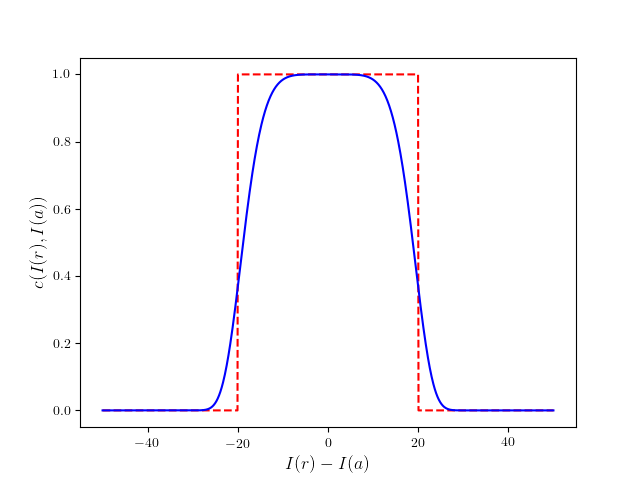
\includegraphics[width=.55\textwidth]{./py/cexp.png}
				\caption{Die Intensitätsdifferenz aufgetragen gegen die Vergleichsfunktionen. Rot: $c_t$, blau: $c_{t,exp}$, $t = 10$.}
			\end{figure}

			In der Praxis ist es häufig von Vorteil statt $c_t$ die Vergleichsfunktion
			$$
				c_{t, exp}(r, r_0) =
					\text{exp}\bigg(-\Big(\frac{I(r) - I(r_0)}{t}\Big)^6\bigg)
			$$
			zu wählen.
			Diese Funktion wird nur annähernd $0$ für große Intensitätsdifferenzen, darum wählen wir zusätzlich $g$ als $\frac{3}{4}$ der Maskengröße. Diese Wahl von $g$ und $c_{t,exp}$ hat zur Folge, dass für Pixel $r$ mit vorher kleinem $A(r)$ nun $A(r) = 0$ gilt. Dies trägt positiv zur Rauschentfernung bei. Die Wirksamkeit dieser Maßnahme ist beispielhaft an Abbildung \ref{fig:lena_first_test} sichtbar.

			\begin{figure}[H]\centering
				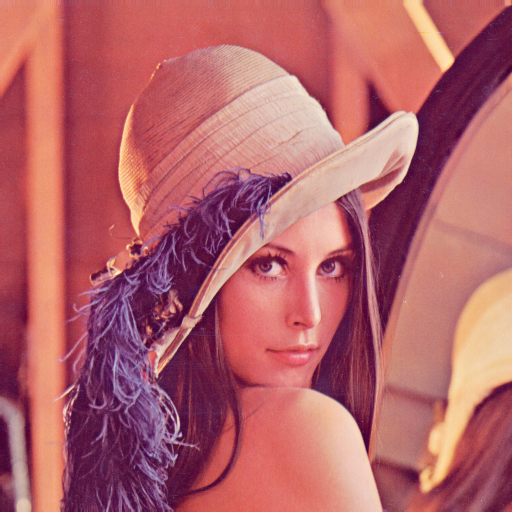
\includegraphics[width=.3\textwidth]{../examples/lena/lena.png}\quad
				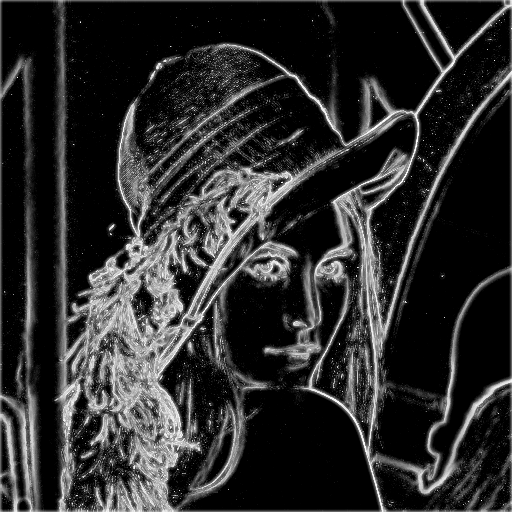
\includegraphics[width=.3\textwidth]{../examples/lena/no-geom_raw.png}\quad
				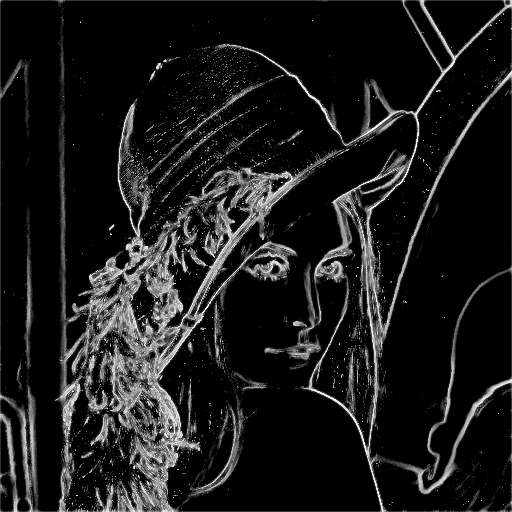
\includegraphics[width=.3\textwidth]{../examples/lena/15_out_raw.png}
				\caption{Ein Testdurchlauf mit $t=15$ und der $7\times 7$ Maske. Ganz links ist das Originalbild. In der Mitte ist $g$ die Maskengröße und $c_t$ die Vergleichsfunktion. $g$ ist rechts $\frac{3}{4}$ der Maskengröße und die Vergleichsfunktion ist $c_{t,exp}$.}
				\label{fig:lena_first_test}
			\end{figure}

			Da dieser Algorithmus von den lokalen Bedingungen jedes Pixels abhängt, kann er nicht durch eine Faltung ausgedrückt werden, wie etwa eine Reihe anderer Filter, darunter der Gaußsche Filter aus \ref{sec:imageproc}, aber auch der Kantendetektor von Canny (siehe \ref{sec:canny}).

		\subsection{Non-Maximum-Suppression I}\label{ssec:nonmax}
			Das oben genannte Prinzip aus Abschnitt \ref{ssec:susan_principle} findet Kanten innerhalb von Bildern, aber die Lokalisation der Kanten könnte besser sein, wie wir in der Abbildung \ref{fig:susan_principle} bereits erkennen konnten. Im Bereich der eigentlichen Kante stellen wir fest, dass die Antwort $A$ ungleich $0$ ist. Um die Kante genauer zu lokalisieren, verwenden wir das Prinzip der Non-Maximum-Suppression, bei der nur die maximale Antwort entlang einer Kante erhalten bleibt. Anders formuliert möchte man die lokal kleinsten USAN finden, daher auch der Name SUSAN (\emph{smallest univalue segment assimilating nucleus}).
			Zu diesem Zweck berechnen wir die Kantenrichtung an jedem Pixel $r_0 = (x_0, y_0)$, für welches $A(x_0, y_0) \neq 0$ gilt, durch eine Fallunterscheidung. Das scheint im ersten Moment fragwürdig, da Pixel an sich keine Richtung haben, sondern die Kanten. Viel mehr ist die Richtung der Kante an der Stelle des jeweiligen Pixel gemeint. Der Einfachheit halber behalten wir uns trotzdem den Begriff der Richtung des Pixels vor. Wir unterscheiden dabei verschiedene Arten von Kanten.

			\begin{figure}[H]
				\begin{center}
					\begin{minipage}{0.5\textwidth}\centering
						\begin{tikzpicture}[fill=black, text=white, color=black]
							\tiny
							\matrix(m)[matrix of nodes, nodes={draw, minimum size = 0.6cm}, nodes in empty cells, column sep=-\pgflinewidth,row sep=-\pgflinewidth]{
								|[fill=white!29!black]|\phantom{H}	&|[fill=white!29!black]|\phantom{H}	&|[fill=white!29!black]|\phantom{H}	&|[fill=white!29!black]|\phantom{H}	&|[fill=white!29!black]|\phantom{H}	&|[fill=white!29!black]|\phantom{H}	&|[fill=white!29!black]|\phantom{H}	&|[fill=white!29!black]|\phantom{H}	\\ 
								|[fill=white!29!black]|\phantom{H}	&|[fill=white!29!black]|\phantom{H}	&|[fill=white!29!black]|\phantom{H}	&|[fill=white!29!black]|\phantom{H}	&|[fill=white!29!black]|\phantom{H}	&|[fill=white!29!black, text=white]|B	&|[fill=white!29!black]|\phantom{H}	&|[fill=white!29!black]|\phantom{H}	\\ 
								|[fill=white!29!black]|\phantom{H}	&|[fill=white!29!black]|\phantom{H}	&|[fill=white!29!black]|\phantom{H}	&|[fill=white!29!black]|\phantom{H}	&|[fill=white!100!black, text=black]|\phantom{H}	&|[fill=white!100!black, text=black]|A	&|[fill=white!100!black, text=black]|\phantom{H}	&|[fill=white!100!black, text=black]|\phantom{H}\\ 
								|[fill=white!29!black]|\phantom{H}	&|[fill=white!29!black]|\phantom{H}	&|[fill=white!29!black]|\phantom{H}	&|[fill=white!29!black]|\phantom{H}	&|[fill=white!100!black, text=black]|\phantom{H}	&|[fill=white!100!black, text=black]|\phantom{H}	&|[fill=white!100!black, text=black]|\phantom{H}	&|[fill=white!100!black, text=black]|\phantom{H}\\ 
								|[fill=white!100!black, text=black]|\phantom{H}	&|[fill=white!100!black, text=black]|\phantom{H}	&|[fill=white!100!black, text=black]|\phantom{H}	&|[fill=white!29!black]|\phantom{H}			&|[fill=white!100!black, text=black]|\phantom{H}	&|[fill=white!100!black, text=black]|\phantom{H}	&|[fill=white!100!black, text=black]|\phantom{H}	&|[fill=white!100!black, text=black]|\phantom{H}	\\ 
								|[fill=white!100!black, text=black]|\phantom{H}	&|[fill=white!100!black, text=black]|\phantom{H}	&|[fill=white!100!black, text=black]|\phantom{H}	&|[fill=white!29!black, text=white]|C		&|[fill=white!100!black, text=black]|\phantom{H}	&|[fill=white!100!black, text=black]|\phantom{H}	&|[fill=white!100!black, text=black]|\phantom{H}	&|[fill=white!100!black, text=black]|\phantom{H}	\\ 
								|[fill=white!100!black, text=black]|\phantom{H}	&|[fill=white!100!black, text=black]|\phantom{H}	&|[fill=white!100!black, text=black]|\phantom{H}	&|[fill=white!29!black]|\phantom{H}			&|[fill=white!100!black, text=black]|\phantom{H}	&|[fill=white!100!black, text=black]|\phantom{H}	&|[fill=white!100!black, text=black]|\phantom{H}	&|[fill=white!100!black, text=black]|\phantom{H}	\\ 
								|[fill=white!100!black, text=black]|\phantom{H}	&|[fill=white!100!black, text=black]|\phantom{H}	&|[fill=white!100!black, text=black]|\phantom{H}	&|[fill=white!29!black]|\phantom{H}			&|[fill=white!100!black, text=black]|\phantom{H}	&|[fill=white!100!black, text=black]|\phantom{H}	&|[fill=white!100!black, text=black]|\phantom{H}	&|[fill=white!100!black, text=black]|\phantom{H}	\\ 
							};				
						\end{tikzpicture}

						Eingangsbild
					\end{minipage}
					\begin{minipage}{0.45\textwidth}\centering
						\begin{tikzpicture}[fill=red]
							\tiny
							\matrix(m)[matrix of nodes, nodes={draw, minimum size = 0.5cm}, nodes in empty cells, column sep=-\pgflinewidth,row sep=-\pgflinewidth]{
								|[fill]|\phantom{H}& |[fill]|\phantom{H}& |[fill]|\phantom{H}\\
								|[fill=green]|\phantom{H}& |[fill=green]|A& |[fill=green]|\phantom{H}\\
								|[fill=green]|\phantom{H}& |[fill=green]|\phantom{H}& |[fill=green]|\phantom{H}\\
							};
						\end{tikzpicture}
						\begin{tikzpicture}[fill=red]
							\tiny
							\matrix(m)[matrix of nodes, nodes={draw, minimum size = 0.5cm}, nodes in empty cells, column sep=-\pgflinewidth,row sep=-\pgflinewidth]{
								|[fill=green]|\phantom{H}& |[fill=green]|\phantom{H}& |[fill=green]|\phantom{H}\\
								|[fill=green]|\phantom{H}& |[fill=green]|B& |[fill=green]|\phantom{H}\\
								|[fill]|\phantom{H}& |[fill]|\phantom{H}& |[fill]|\phantom{H}\\
							};
						\end{tikzpicture}

						Inter-Pixel-Fall
						\vspace{1em}

						\begin{tikzpicture}[fill=red]
							\tiny
							\matrix(m)[matrix of nodes, nodes={draw, minimum size = 0.5cm}, nodes in empty cells, column sep=-\pgflinewidth,row sep=-\pgflinewidth]{
								|[fill]|\phantom{H}& |[fill=green]|\phantom{H}& |[fill]|\phantom{H}\\
								|[fill]|\phantom{H}& |[fill=green]|C& |[fill]|\phantom{H}\\
								|[fill]|\phantom{H}& |[fill=green]|\phantom{H}& |[fill]|\phantom{H}\\
							};
						\end{tikzpicture}
						\begin{tikzpicture}[fill=red]
							\tiny
							\matrix(m)[matrix of nodes, nodes={draw, minimum size = 0.5cm}, nodes in empty cells, column sep=-\pgflinewidth,row sep=-\pgflinewidth]{
								|[fill=green]|\phantom{H}& |[fill]|\phantom{H}& |[fill]|\phantom{H}\\
								|[fill]|\phantom{H}& |[fill=green]|D& |[fill]|\phantom{H}\\
								|[fill]|\phantom{H}& |[fill]|\phantom{H}& |[fill=green]|\phantom{H}\\
							};
						\end{tikzpicture}
						\begin{tikzpicture}[fill=red]
							\tiny
							\matrix(m)[matrix of nodes, nodes={draw, minimum size = 0.5cm}, nodes in empty cells, column sep=-\pgflinewidth,row sep=-\pgflinewidth]{
								|[fill]|\phantom{H}& |[fill]|\phantom{H}& |[fill=green]|\phantom{H}\\
								|[fill]|\phantom{H}& |[fill=green]|E& |[fill]|\phantom{H}\\
								|[fill=green]|\phantom{H}& |[fill]|\phantom{H}& |[fill]|\phantom{H}\\
							};
						\end{tikzpicture}

						Intra-Pixel-Fall


					\end{minipage}

					\caption{Inter-Pixel-Fall und Intra-Pixel-Fall für die $3\times 3$ Maske: Die drei rechts abgebildeten USAN wurden durch Wahl des Nukleus an den mit A, B und C markierten Stellen im Eingangsbild ausgewertet. Die grün markierten Pixel stehen für Teile der USAN. Die Nuklei D und E gelten nur der weiteren Illustration von Möglichkeiten und sind nicht im Eingangsbild vorzufinden.}
					\label{fig:inter-intra}
				\end{center}
			\end{figure}


			Für die Fallunterscheidung zwischen den Pixeln benötigen wir das sogenannte \emph{center of gravity} oder Gravitationszentrum einer jeden USAN:
				$$ \text{COG}(r_0) := \frac	{\sum_r r\,c(r,r_0)} {\sum_r c(r,r_0)} = \frac	{\sum_r r\,c(r,r_0)} {n(r_0)} \in \mathbb{R}^2.$$
			Das $\text{COG}(r_0)$ ist die gewichtete Summe der durch $c \in \{c_t, c_{t,exp}\}$ bedingt ähnlichen Pixel; also in Relation zu $r_0$ die Richtung, in der die meisten ähnlichen Pixel in der Maske sind.
			Wir betrachten zum Beispiel die Abbildung \ref{fig:inter-intra} mit der $3\times3$ Maske, $c = c_t$ und unter der Annahme, dass $A := (5,2)$. In der Abbildung \ref{fig:inter-intra} stehen die grün markierten Pixel jeweils für Pixel, die in der USAN liegen. Die roten Pixel liegen außerhalb der USAN. Die Mitte ist der Nukleus der Maske. Es gilt:
			\begin{align*}
				\text{COG}(\text{A})
				= &\;\frac{\sum_r r\,c(r,\text{A})} {\sum_r c(r, \text{A})} \\
				= &\;0\begin{bmatrix}4\\1\end{bmatrix} + 0\begin{bmatrix}5\\1\end{bmatrix} + 0\begin{bmatrix}6\\1\end{bmatrix} \\
				+ &\;1\begin{bmatrix}4\\2\end{bmatrix} + 1\begin{bmatrix}5\\2\end{bmatrix} + 1\begin{bmatrix}6\\2\end{bmatrix} \\
				+ &\;1\begin{bmatrix}4\\3\end{bmatrix} + 1\begin{bmatrix}5\\3\end{bmatrix} + 1\begin{bmatrix}6\\3\end{bmatrix} = \begin{bmatrix}5\\2.5\end{bmatrix}.
			\end{align*}

			In Fällen wie bei dem Pixel A können wir nun die Richtung folgendermaßen bestimmen: Der Vektor zwischen dem Nukleus $\text{A} := (\text{A}_x, \text{A}_y)$ und seinem Gravitationszentrum $\text{COG}(\text{A}) := (\text{COG}_x(\text{A}), (\text{COG}_y(\text{A}))$ ist gegeben durch $$\text{COG}(\text{A}) - \text{A} := \begin{bmatrix}\text{COG}_x(\text{A}) - \text{A}_x \\ \text{COG}_y(\text{A}) - \text{A}_y\end{bmatrix}.$$
			Der gesuchte Vektor soll nun senkrecht auf $\text{COG}(\text{A}) - \text{A}$ stehen und damit die Richtung der Kante beschreiben. Es gilt:
			$$\begin{bmatrix}\text{COG}_y(\text{A}) - \text{A}_y \\ \text{COG}_x(\text{A}) - \text{A}_x\end{bmatrix} \bot \; \left(\text{COG}(\text{A}) - \text{A}\right).$$

			Wir beobachten allerdings für das Pixel C in der Abbildung \ref{fig:inter-intra} und den gleichen Bedingungen wie bei der vorherigen Berechnung, dass $\text{COG}(\text{C}) = \text{C}$. Da keine Distanz zwischen $\text{COG}(\text{C})$ und C ist, kann die Richtung der Kante mit dem oben genannten Verfahren nicht ermittelt werden. Bei kleineren Distanzen zwischen einem Pixel $r$ und seinem $\text{COG}(r)$ wird das Verfahren zunehmend ungenau. Stattdessen nutzen wir eine Art Stichprobenvarianz in $x$- und $y$-Richtung folgendermaßen: Summiere für alle Pixel in der Maske $r = (x, y)$ und den Nukleus $r_0 = (x_0, y_0)$ für $c \in \{c_t, c_{t,exp}\}$
			\begin{align*}
				Var_{x}(r_0) &:= \frac{1}{N}\sum_{r=(x,y)} (x-x_0)^2 \, c(r,r_0), \\
				Var_{y}(r_0) &:= \frac{1}{N}\sum_{r=(x,y)} (y-y_0)^2 \, c(r,r_0),
 			\end{align*}
 			wobei $N$ die Anzahl der Pixel ist, über die iteriert wird.
 			Die Varianz ist ein Maß dafür, wie weit die Pixel, die in der USAN liegen, durchschnittlich vom "Mittelwert" (in diesem Fall dem Nukleus $r_0$) in $x$- beziehungsweise $y$-Richtung abweichen. Im Falle des Pixels $\text{C} = (3,5)$ mit der $3\times3$ Maske und der $c = c_t$ sind die Varianzen gegeben durch
 			\begin{align*}
 				N \; Var_x(\text{C}) 	=\; &(2-3)^2 \cdot 0 \;+\; (3-3)^2 \cdot 1 \;+\; (4-3)^2 \cdot 0  \\
 										+\; &(2-3)^2 \cdot 0 \;+\; (3-3)^2 \cdot 1 \;+\; (4-3)^2 \cdot 0  \\
 										+\; &(2-3)^2 \cdot 0 \;+\; (3-3)^2 \cdot 1 \;+\; (4-3)^2 \cdot 0  = 0, \\
 										\\
 				N \; Var_y(\text{C}) 	=\; &(4-5)^2 \cdot 0 \;+\; (4-5)^2 \cdot 1 \;+\; (4-5)^2 \cdot 0  \\
 										+\; &(5-5)^2 \cdot 0 \;+\; (5-5)^2 \cdot 1 \;+\; (5-5)^2 \cdot 0  \\
 										+\; &(6-5)^2 \cdot 0 \;+\; (6-5)^2 \cdot 1 \;+\; (6-5)^2 \cdot 0  = 2. \\& 
 			\end{align*}
 			
 			Wie im ersten Fall können wir nun die Richtung des Vektors $\frac{Var_x(\text{C})}{Var_y(\text{C})}$ bestimmen. Der normierende Faktor $N$ der Stichprobenvarianz fällt dabei weg. Angenommen eine diagonale Kante liegt vor.
 			Dann sehen wir, dass $Var_x(r_0) \approx Var_y(r_0)$. Ob eine \glqq positiv diagonale\grqq{} oder \glqq negativ diagonale\grqq{} Kante vorliegt (also eine von links unten nach rechts oben oder eine von rechts unten nach links oben), entscheidet nun ein Vorzeichen, welches wir aufgrund von $Var_x > 0$ und $Var_y > 0$ nicht haben.
 			Das Vorzeichen können wir allerdings mithilfe folgender Gleichung berechnen:
 			$$ Var_{x,y}(r_0) = \sum_{r=(x,y)} (x-x_0) \, (y-y_0) \, c_t(r,r_0).$$
 			Diese \glqq gemischte Varianz\grqq{} trägt die Information über die Richtung der diagonalen Kante im Vorzeichen.
 			Man betrachte zum Beispiel die beiden diagonalen Kanten D und E unter den gleichen Voraussetzungen wie C:
 			 \begin{align*}
 				N \; Var_x(\text{D}) &= N \; Var_x(\text{E}) = 2 \\
 				N \; Var_y(\text{D}) &= N \; Var_y(\text{E}) = 2 \\
 				\text{sgn}(Var_{x,y}(\text{D})) 	&=\;\text{sgn}\bigg((-1) \cdot (-1)+ 0 \cdot 0 +1 \cdot 1\bigg) = 1\\
 				\text{sgn}(Var_{x,y}(\text{E}))		&=\;\text{sgn}\bigg((-1) \cdot 1+ 0 \cdot 0 +1 \cdot (-1)\bigg) = -1.\\
 			\end{align*}
 			

 			Für jeden Nukleus gilt: Falls das COG nah am Nukleus liegt und viele Pixel in der USAN liegen, so sprechen wir vom Inter-Pixel-Fall. Der Inter-Pixel-Fall liegt nämlich vor, wenn eine Kante zwischen zwei Pixeln liegt. Hier benutzen wir die Berechnung der Richtung über das Gravitationszentrum. Der Intra-Pixel-Fall hingegen liegt vor, wenn ein Pixel genau auf der Kante liegt. Hier benutzen wir die Stichprobenvarianz. Zusammenfassend berechnen wir für jedes Pixel $r_0$ im Bild folgendermaßen die Kantenrichtung $D(r_0)$:
			\begin{enumerate}
				\item \textbf{Inter-Pixel:}

				\noindent Falls die Größe der USAN größer ist als der Maskendurchmesser und die Distanz zwischen $\text{COG}(r_0)$ und $r_0=(x_0, y_0)$ größer als $1$ Pixel ist, so ist die Richtung $D(r_0)$ gegeben durch
				$$ D(r_0) = \begin{cases}
					\text{arctan}\bigg(
						\frac{x_0 - \text{COG}_x(r_0)}
						{y_0 - \text{COG}_y(r_0)}
					\bigg) & \text{falls } \text{COG}_y(r_0) \neq y_0, \\
					
					\frac{\pi}{2} & \text{sonst.}
				\end{cases} $$

				\item \textbf{Intra-Pixel:}
				
				\noindent Andernfalls müssen wir die Stichprobenvarianzen der USAN folgendermaßen berechnen. Über alle Pixel $r = (x, y)$ in der Maske und $r_0 = (x_0, y_0)$ summieren wir
				\begin{align*}
					N \; Var_x(r_0) &:= \sum_r (x-x_0)^2 \, c_t(r,r_0), \\
					N \; Var_y(r_0) &:= \sum_r (y-y_0)^2 \, c_t(r,r_0), \\
					\sigma 	&:= -\text{sgn}\bigg(\sum_r (x-x_0) \, (y-y_0) \, c_t(r,r_0)\bigg).
				\end{align*}
				Dabei ergibt sich die Kantenrichtung als
				$$ D(r_0) = \begin{cases}
						\sigma \, \text{arctan} \, \frac{Var_y(r_0)}{Var_x(r_0)} 	&	\text{falls } Var_x(r_0) \neq 0 \text{ und } \sigma \neq 0, \\
						\frac{\pi}{2}												&	\text{falls } \sigma = 0 \text{ und } Var_x(r_0) < Var_y(r_0)\\
						& \text{oder falls } Var_x(r_0) = 0,\\
						0												&	\text{sonst}.
					\end{cases}$$
			\end{enumerate}

			\begin{figure}[H]\centering
				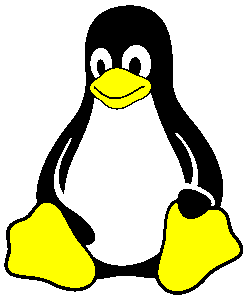
\includegraphics[width=.4\textwidth]{../examples/tux/tux.png}\quad
				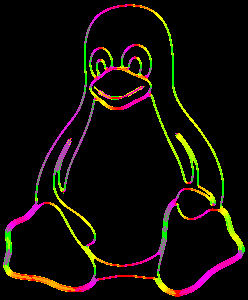
\includegraphics[width=.4\textwidth]{../examples/tux/15_out_heat.png}\quad
				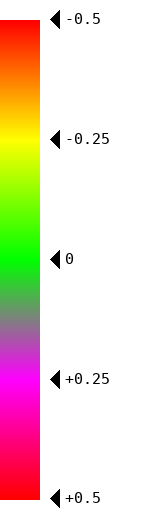
\includegraphics[width=.14\textwidth]{assets/heatmap-strip/strip.png}
				\caption{Ein Testdurchlauf für das Berechnen der Richtungen mit $t=15$. Links ist das Eingangsbild. Rechts ist die Kantenrichtung für jedes Pixel abgebildet. Die Zahlenwerte können an der Skala abgelesen werden und sind als Vielfache von $\pi$ angegeben.}
				\label{fig:directions_test}
			\end{figure}

			Für Pixel außerhalb des Definitionsbereiches $r \notin [0, B-1]_\mathbb{Z} \times [0, H-1]_\mathbb{Z}$ legen wir für diese Berechnungen die gleichen Randbedingungen fest, die wir auch schon für den Hauptteil des Algorithmus in Sektion \ref{ssec:susan_principle} festgelegt haben.

			Die Berechnungen für die jeweiligen Kantenrichtungen an jedem Pixel werden in der Implementation gleichzeitig mit den Berechnungen für das SUSAN-Prinzip durchgeführt. Auf diese Weise müssen $c$ und $n$ an jeder Stelle nur einmal berechnet werden.

			\begin{figure}[H]\centering
					\begin{tikzpicture}[fill=white, text=black]
					\tiny
					\matrix(m)[matrix of nodes, nodes={draw, minimum size = .6cm}, column sep=-\pgflinewidth,row sep=-\pgflinewidth]{
						|[fill]|$\cdot$ & |[fill]|$\cdot$ & |[fill]|$\cdot$ & |[fill]|$\cdot$ & |[fill]|$\downarrow$ & |[fill]|$\downarrow$ & |[fill]|$\downarrow$ & |[fill]|$\cdot$ & |[fill]|$\cdot$ & |[fill]|$\cdot$ & |[fill]|$\cdot$ \\
						|[fill]|$\cdot$ & |[fill]|$\cdot$ & |[fill]|$\cdot$ & |[fill]|$\cdot$ & |[fill]|$\downarrow$ & |[fill]|$\downarrow$ & |[fill]|$\downarrow$ & |[fill]|$\cdot$ & |[fill]|$\cdot$ & |[fill]|$\cdot$ & |[fill]|$\cdot$ \\
						|[fill]|$\cdot$ & |[fill]|$\cdot$ & |[fill]|$\cdot$ & |[fill]|$\cdot$ & |[fill]|$\downarrow$ & |[fill]|$\downarrow$ & |[fill]|$\downarrow$ & |[fill]|$\cdot$ & |[fill]|$\cdot$ & |[fill]|$\cdot$ & |[fill]|$\cdot$ \\
						|[fill]|$\cdot$ & |[fill]|$\cdot$ & |[fill]|$\cdot$ & |[fill]|$\cdot$ & |[fill]|$\downarrow$ & |[fill]|$\downarrow$ & |[fill]|$\downarrow$ & |[fill]|$\cdot$ & |[fill]|$\cdot$ & |[fill]|$\cdot$ & |[fill]|$\cdot$ \\
						|[fill]|$\cdot$ & |[fill]|$\cdot$ & |[fill]|$\cdot$ & |[fill]|$\cdot$ & |[fill]|$\downarrow$ & |[fill]|$\downarrow$ & |[fill]|$\downarrow$ & |[fill]|$\cdot$ & |[fill]|$\cdot$ & |[fill]|$\cdot$ & |[fill]|$\cdot$ \\
						|[fill]|$\cdot$ & |[fill]|$\cdot$ & |[fill]|$\cdot$ & |[fill]|$\cdot$ & |[fill]|$\downarrow$ & |[fill]|$\downarrow$ & |[fill]|$\downarrow$ & |[fill]|$\cdot$ & |[fill]|$\cdot$ & |[fill]|$\cdot$ & |[fill]|$\cdot$ \\
						|[fill]|$\cdot$ & |[fill]|$\cdot$ & |[fill]|$\cdot$ & |[fill]|$\cdot$ & |[fill]|$\downarrow$ & |[fill]|$\downarrow$ & |[fill]|$\downarrow$ & |[fill]|$\cdot$ & |[fill]|$\cdot$ & |[fill]|$\cdot$ & |[fill]|$\cdot$ \\
						|[fill]|$\cdot$ & |[fill]|$\cdot$ & |[fill]|$\cdot$ & |[fill]|$\cdot$ & |[fill]|$\downarrow$ & |[fill]|$\downarrow$ & |[fill]|$\downarrow$ & |[fill]|$\cdot$ & |[fill]|$\cdot$ & |[fill]|$\cdot$ & |[fill]|$\cdot$ \\
						|[fill]|$\cdot$ & |[fill]|$\cdot$ & |[fill]|$\cdot$ & |[fill]|$\cdot$ & |[fill]|$\downarrow$ & |[fill]|$\downarrow$ & |[fill]|$\downarrow$ & |[fill]|$\cdot$ & |[fill]|$\cdot$ & |[fill]|$\cdot$ & |[fill]|$\cdot$ \\
						|[fill]|$\cdot$ & |[fill]|$\cdot$ & |[fill]|$\cdot$ & |[fill]|$\cdot$ & |[fill]|$\downarrow$ & |[fill]|$\downarrow$ & |[fill]|$\downarrow$ & |[fill]|$\cdot$ & |[fill]|$\cdot$ & |[fill]|$\cdot$ & |[fill]|$\cdot$ \\
						|[fill]|$\cdot$ & |[fill]|$\cdot$ & |[fill]|$\cdot$ & |[fill]|$\cdot$ & |[fill]|$\downarrow$ & |[fill]|$\downarrow$ & |[fill]|$\downarrow$ & |[fill]|$\cdot$ & |[fill]|$\cdot$ & |[fill]|$\cdot$ & |[fill]|$\cdot$ \\
					};
					\normalsize
				\end{tikzpicture}
				\begin{tikzpicture}[fill=black, text=white]
					\tiny
					\matrix(m)[matrix of nodes, nodes={draw, minimum size = .6cm}, column sep=-\pgflinewidth,row sep=-\pgflinewidth]{
						|[fill=white!0!black]|0	&|[fill=white!0!black]|0	&|[fill=white!0!black]|0&|[fill=white!0!black]|0	&|[fill=white!0!black]|0	&|[fill=white!100!black, text=black]|255	&|[fill=white!0!black]|0	&|[fill=white!0!black]|0	&|[fill=white!0!black]|0	&|[fill=white!0!black]|0	&|[fill=white!0!black]|0	\\ 
						|[fill=white!0!black]|0	&|[fill=white!0!black]|0	&|[fill=white!0!black]|0&|[fill=white!0!black]|0	&|[fill=white!0!black]|0	&|[fill=white!100!black, text=black]|255	&|[fill=white!0!black]|0	&|[fill=white!0!black]|0	&|[fill=white!0!black]|0	&|[fill=white!0!black]|0	&|[fill=white!0!black]|0	\\ 
						|[fill=white!0!black]|0	&|[fill=white!0!black]|0	&|[fill=white!0!black]|0&|[fill=white!0!black]|0	&|[fill=white!0!black]|0	&|[fill=white!100!black, text=black]|255	&|[fill=white!0!black]|0	&|[fill=white!0!black]|0	&|[fill=white!0!black]|0	&|[fill=white!0!black]|0	&|[fill=white!0!black]|0	\\ 
						|[fill=white!0!black]|0	&|[fill=white!0!black]|0	&|[fill=white!0!black]|0&|[fill=white!0!black]|0	&|[fill=white!0!black]|0	&|[fill=white!100!black, text=black]|255	&|[fill=white!0!black]|0	&|[fill=white!0!black]|0	&|[fill=white!0!black]|0	&|[fill=white!0!black]|0	&|[fill=white!0!black]|0	\\ 
						|[fill=white!0!black]|0	&|[fill=white!0!black]|0	&|[fill=white!0!black]|0&|[fill=white!0!black]|0	&|[fill=white!0!black]|0	&|[fill=white!100!black, text=black]|255	&|[fill=white!0!black]|0	&|[fill=white!0!black]|0	&|[fill=white!0!black]|0	&|[fill=white!0!black]|0	&|[fill=white!0!black]|0	\\ 
						|[fill=white!0!black]|0	&|[fill=white!0!black]|0	&|[fill=white!0!black]|0&|[fill=white!0!black]|0	&|[fill=white!0!black]|0	&|[fill=white!100!black, text=black]|255	&|[fill=white!0!black]|0	&|[fill=white!0!black]|0	&|[fill=white!0!black]|0	&|[fill=white!0!black]|0	&|[fill=white!0!black]|0	\\ 
						|[fill=white!0!black]|0	&|[fill=white!0!black]|0	&|[fill=white!0!black]|0&|[fill=white!0!black]|0	&|[fill=white!0!black]|0	&|[fill=white!100!black, text=black]|255	&|[fill=white!0!black]|0	&|[fill=white!0!black]|0	&|[fill=white!0!black]|0	&|[fill=white!0!black]|0	&|[fill=white!0!black]|0	\\ 
						|[fill=white!0!black]|0	&|[fill=white!0!black]|0	&|[fill=white!0!black]|0&|[fill=white!0!black]|0	&|[fill=white!0!black]|0	&|[fill=white!100!black, text=black]|255	&|[fill=white!0!black]|0	&|[fill=white!0!black]|0	&|[fill=white!0!black]|0	&|[fill=white!0!black]|0	&|[fill=white!0!black]|0	\\ 
						|[fill=white!0!black]|0	&|[fill=white!0!black]|0	&|[fill=white!0!black]|0&|[fill=white!0!black]|0	&|[fill=white!0!black]|0	&|[fill=white!100!black, text=black]|255	&|[fill=white!0!black]|0	&|[fill=white!0!black]|0	&|[fill=white!0!black]|0	&|[fill=white!0!black]|0	&|[fill=white!0!black]|0	\\ 
						|[fill=white!0!black]|0	&|[fill=white!0!black]|0	&|[fill=white!0!black]|0&|[fill=white!0!black]|0	&|[fill=white!0!black]|0	&|[fill=white!100!black, text=black]|255	&|[fill=white!0!black]|0	&|[fill=white!0!black]|0	&|[fill=white!0!black]|0	&|[fill=white!0!black]|0	&|[fill=white!0!black]|0	\\ 
						|[fill=white!0!black]|0	&|[fill=white!0!black]|0	&|[fill=white!0!black]|0&|[fill=white!0!black]|0	&|[fill=white!0!black]|0	&|[fill=white!100!black, text=black]|255	&|[fill=white!0!black]|0	&|[fill=white!0!black]|0	&|[fill=white!0!black]|0	&|[fill=white!0!black]|0	&|[fill=white!0!black]|0	\\ 
					};
					\normalsize
				\end{tikzpicture}
				\caption{Eingangsbild wie in Abbildung \ref{fig:noborder}. Links sind die Kantenrichtungen abgebildet und klassifiziert wie wir noch in Sektion \ref{ssec:nonmax_implem} besprechen werden. Auf dem rechten Bild wurde die Kante pixelgenau durch Non-Maximum-Suppression lokalisiert.}
			\end{figure}

			Die Richtung muss nur für diejenigen Pixel $(i,j)$ bestimmt werden, für die $A(i,j) > 0$ gilt. Ist die Richtung der Kante bestimmt, so können wir die lokalen Maxima von $A$ entlang der Richtung, die senkrecht zur Kantenrichtung steht, erhalten. Alles, was kein lokales Maximum entlang dieser Richtung ist, wird verworfen (also wird die Antwort an dieser Stelle $= 0$ gesetzt). Wir erhalten so ein neues Bild. In Sektion \ref{ssec:nonmax_implem} wird darauf eingegangen, wie genau dieser Prozess implementiert wurde.
			
			Die dort vorgestellte Prozedur kategorisiert jedes Pixel nach der generellen Richtung jeder Kante mit $\frac{\pi}{4}$ Genauigkeit. Senkrecht zu dieser Richtung wird dann nur das Maximum der direkten Nachbarschaft erhalten, der Rest wird aus dem Kantenbild entfernt (also $=0$ gesetzt).

			\begin{figure}[H]\centering
				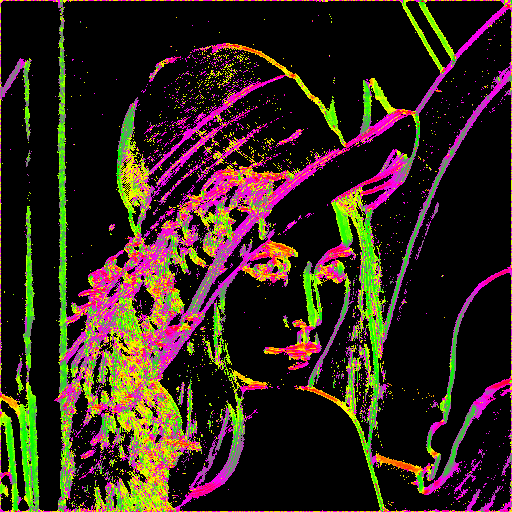
\includegraphics[width=.3\textwidth]{../examples/lena/15_out_heat.png}\quad
				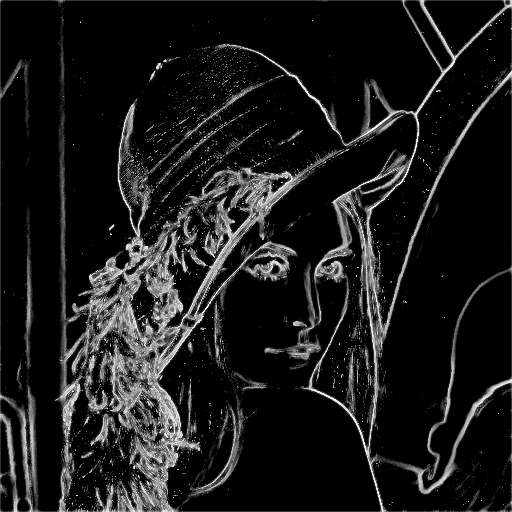
\includegraphics[width=.3\textwidth]{../examples/lena/15_out_raw.png}\quad
				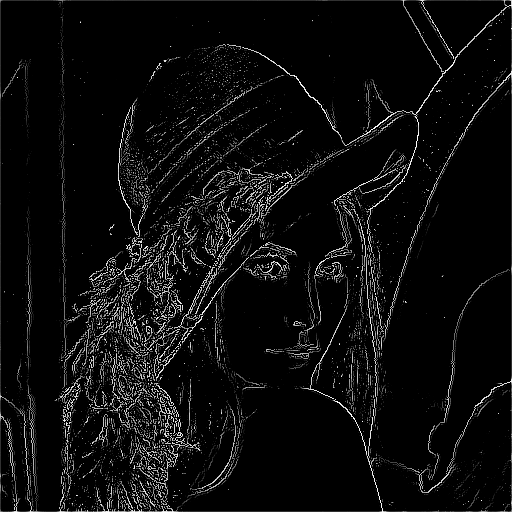
\includegraphics[width=.3\textwidth]{../examples/lena/15_out_nonmax_supp.png}

				\caption{Wie Abbildung \ref{fig:lena_first_test}. Links das Bild mit den Kantenrichtungen (Skala wie in Abbildung \ref{fig:directions_test}). In der Mitte das Bild nach dem prinzipiellen SUSAN-Schritt. Das Bild rechts ist nach der Non-Maximum-Suppression.}
				\label{fig:lena_nonmax_supp}
			\end{figure}

			Die Non-Maximum-Suppression unterdrückt in unserem Beispiel tatsächlich alle diejenigen Pixel, die keine lokalen Maxima in der Richtung senkrecht zur Kante sind. Auch für größere Bilder erzielt die Non-Maximum-Suppression den erwünschten Effekt, siehe Abbildung \ref{fig:lena_nonmax_supp}.


		\subsection{Ausdünnen}\label{ssec:thinout}
			Da viele digitale Bilder eingangs mit Rauschen behaftet sind, ist es manchmal hilfreich, einzelne Antworten zu entfernen und dafür andere hinzuzufügen. Zu diesem Zwecke empfiehlt \cite{SUSAN}, dass man einige der Kanten ausdünnt. Dieser Vorgang wird genauer in \cite{thinout} beschrieben.
			Es wird erneut über das ganze Bild iteriert. Jedes Pixel $(i,j)$ mit einer Antwort $A(i,j) > 0$ wird auf die Anzahl seiner direkten Nachbarn mit $A(x,y) > 0$ überprüft. Als direkte Nachbarschaft werden die acht nächsten Pixel bezeichnet, siehe dazu die $3\times 3$ Maske in Abbildung \ref{fig:def_masken}. Angenommen, das Pixel hat
			\begin{itemize}
				\item \textbf{0 Nachbarn:}
					Entferne die Antwort des Pixels.
				\item \textbf{1 Nachbar:}
					Überprüfe, ob in einer Reichweite von 3 Pixeln eine Linie mit der gleichen Richtung existiert. Falls ja, verbinde die Pixel miteinander.
				\item \textbf{2 Nachbarn:}
					Falls das Pixel benachbart zu einer diagonalen Linie ist, entferne es.
					Falls das Pixel außerhalb einer sonst horizontalen oder vertikalen Linie liegt, verschiebe die Antwort des Pixels in die Lücke der vertikalen oder horizontalen Linie.
				\item \textbf{3 Nachbarn:}
					Falls die drei Nachbarn in einer Linie liegen, entferne die Antwort des Pixels.
			\end{itemize}

			Im Testbild der Abbildung \ref{fig:thinout_test} erkennt man die Funktionsweise in allen vier oben genannten Fällen.

			\begin{figure}[H]\centering
				
\includegraphics[width=0.45\textwidth]{./assets/thinout/out_nonmax_supp.png}\quad
				
\includegraphics[width=0.45\textwidth]{./assets/thinout/out_thinned.png}

				\vspace{0.5em}

				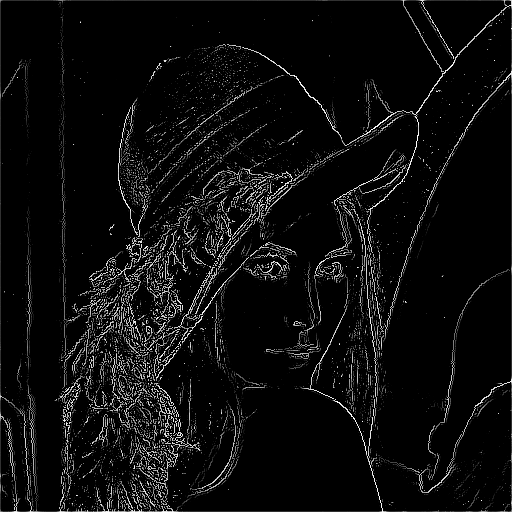
\includegraphics[width=0.45\textwidth]{../examples/lena/15_out_nonmax_supp.png}\quad
				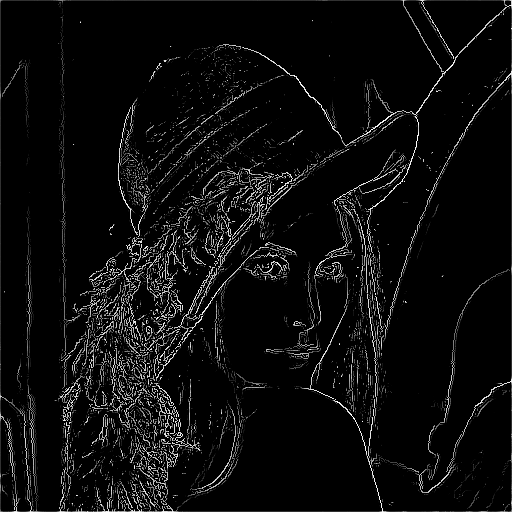
\includegraphics[width=0.45\textwidth]{../examples/lena/15_out_thinned.png}
				\caption{Links: Kantenbilder nach der Non-Maximum-Suppression. Rechts: Kantenbilder nach dem Ausdünnen.}
				\label{fig:thinout_test}
			\end{figure}

			Laut der zitierten Quelle \cite{thinout} soll eigentlich auch für die Fälle mit mehr als 3 Nachbarn gesorgt werden. Allerdings ist eine Vorhersage über Nachbarschaften mit 4 oder mehr Nachbarn relativ schwierig. Es müssten mehrere Nachbarn zur genauen Beurteilung der jeweiligen Situation herangezogen werden.
			Der Ausdünnungsschritt wird in \cite{SUSAN} als optional bezeichnet und seine Wirkung ist fragwürdig und nicht belegt. Es besteht gerade bei feinen Strukturen mit vielen, nah beieinanderliegenden Kanten die Möglichkeit, dass der Schritt richtig identifizierte Stellen einer Kante aus der Antwort unterdrückt und im Gegenzug Kanten verbindet, die nicht verbunden sind.

		\subsection{Der SUSAN-Eckendetektor}\label{ssec:corner_detector}
			In \cite{SUSAN} wird zusätzlich ein Verfahren beschrieben, mit welchem sich durch das SUSAN-Prinzip Ecken finden lassen. Dieser Eckendetektor basiert darauf, dass der SUSAN-Kantendetektor an Ecken stärkere Antworten liefert als an Kanten (siehe auch Abbildung \ref{fig:susan_principle_corners}).
			Wir erinnern uns an den Algorithmus aus Sektion \ref{ssec:susan_principle}:
			$$
				A(r_0) = \text{max}\{0, g - n(r_0)\},\;
				n(r_0) = \sum_r c_t(r, r_0),\;
				c_t(r, r_0) =
					\begin{cases}
						1 	& \text{falls } |I(r) - I(r_0)| \leq t, 	\\
						0 	& \text{sonst.}
					\end{cases}
			$$
			Um nur vergleichsweise starke Antworten zu erhalten, benutzen wir statt dem bisherigen geometrischen Schwellenwert $g$ einen niedrigeren Wert. Im Beispiel in Abbildung \ref{fig:corner_test} wurde ein Wert von $\frac{1}{4}$ der Maskengröße verwendet.

			Danach finden sich immer noch viele falsch positive Antworten. Um diese zu vermeiden, überprüft man, ob die jeweiligen Kandidaten mit einer Kante zusammenhängen. Dies gelingt durch das Erzwingen folgender Regeln für jede Ecke:

			\begin{enumerate}
				\item Die Entfernung zwischen Gravitationszentrum und Nukleus muss groß genug sein.
				\item Jedes Pixel in der Maske, welches sich auf gerader Strecke zwischen Nukleus und Gravitationszentrum befindet, muss in der USAN des Nukleus enthalten sein.
				\item Alle Antworten $A(r)$, die kein lokales Maximum in einer $5\times 5$ Maske sind, sollen entfernt werden.
			\end{enumerate}

			Die Entfernung zwischen Gravitationszentrum und Nukleus sichert ab, dass die Richtung der Kante sich an der Ecke ändert. Punkt zwei prüft den räumlichen Zusammenhang von Ecken und Kanten. Der dritte Punkt gleicht vom Prinzip der Non-Maximum-Suppression, allerdings muss bei Ecken keine Richtung festgestellt werden.

			\begin{figure}[H]\centering
				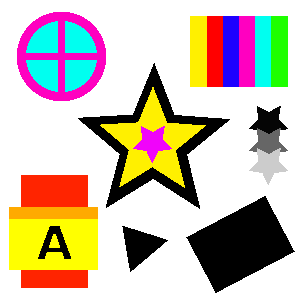
\includegraphics[width=0.45\textwidth]{../examples/original/original.png}\quad
				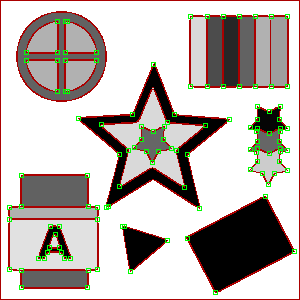
\includegraphics[width=0.45\textwidth]{../examples/original/test_overlay.png}
				\caption{Links das Eingangsbild, rechts sind Kanten und Ecken markiert. Die Ecken sind grün umrahmt wohingegen die Kanten rot übergezeichnet sind. Für $g$ wurde hier $\frac{3}{4}$ der Maskengröße verwendet. Der Mindestabstand zwischen Nukleus und Gravitationszentrum einer jeden USAN ist hier $\sqrt{2}$.}
				\label{fig:corner_test}
			\end{figure}

		\section{Implementation}\label{sec:implementation}
		Meine persönliche Implementation ist in Python 3 erfolgt. Die Software ist abhängig von den folgenden Python 3 Paketen:
		\begin{itemize}
			\item \texttt{pillow}, eine Bibiliothek für Bildverarbeitung \cite{pillow},
			\item \texttt{numpy}, eine Bibliothek für wissenschaftliches Rechnen \cite{numpy},
			\item \texttt{multiprocessing} eine Bibiliothek für prozessbasierte Parallelisierung \cite{multiprocessing}.
		\end{itemize}
		Die Software ist verfügbar unter \cite{mysoftware}. In der Klasse \texttt{Susan.py} befindet sich der vollständige Kantendetektor. Er lässt sich in Python 3 per Anweisung \texttt{import Susan} nutzen. Dazu erzeugt man ein Objekt der \texttt{Susan}-Klasse und übergibt eine Bilddatei. Danach ruft man auf dem Objekt die Funktion \texttt{detect\_edges\_mp} mit dem Parameter $t$, dem Grenzwert aus Abschnitt \ref{ssec:susan_principle}, auf.

		\begin{figure}[H] \centering
			\begin{lstlisting}[language=Python]
	import Susan

	t = 15
	S = Susan("lena.png")
	S.detect_edges_mp(t)
			\end{lstlisting}
		\caption{Nutzen der Python 3 Applikation}
		\label{fig:minimal-working-example}
		\end{figure}

		Es können weiterhin folgende Parameter übergeben werden:
		\begin{center}
			\begin{tabular}{|l|l|l|l|}
				\hline
				\textbf{Name} 		& \textbf{Beschreibung} 	& \textbf{Datentyp}							& \textbf{Standardwert}	\\
				\hline
				\texttt{t}			& Grenzwert	für $c_t$		& Ganzzahl, $t \in [1,255]_\mathbb{N}$		& -\\
				\hline
				\texttt{filename}	& Ausgabepfad				& Zeichenkette								& \texttt{"{}out.png"}\\
				\hline
				\texttt{nms}		& Non-Maximum-				& Boolesch									& \texttt{True}\\
									& Suppression & & \\
				\hline
				\texttt{heatmap}	& Ausgabe der Richtungen 	& Boolesch									& \texttt{False}\\
				\hline
				\texttt{geometric}	& Schwache Antworten 		& Boolesch 									& \texttt{True} \\
									& unterdrücken & & \\
				\hline
				\texttt{corners}	& Ecken finden				& Boolesch									& \texttt{False} \\
				\hline
				\texttt{overlay}	& Überlagerungsbild 		& Boolesch									& \texttt{True} \\
									& erzeugen & & \\
				\hline
			\end{tabular}
		\end{center}

		Beim Paramater \texttt{heatmap} werden die Richtungen als Bild ausgegeben, dabei korrespondieren die Richtungen zu Farben, genau so wie wir es schon in den Abbildungen zu Abschnitt \ref{ssec:nonmax} sehen konnten.
		Falls \texttt{geometric} auf \texttt{True} gesetzt ist, so wird $g$ als $\frac{3}{4}$ der Maskengröße gewählt. Andernfalls ist $g$ gleich der Maskengröße, wie im Abschnitt \ref{ssec:susan_principle}.
		Die Option \texttt{overlay} erzeugt ein Bild, auf dem Kanten in rot nachgezeichnet und Ecken von grünen Kästen umrahmt werden, wie in Abbildung \ref{fig:corner_test}.

			\subsection{Vergleichsfunktion}
				Zu Gunsten der Effizienz habe ich für die Vergleichsfunktion eine Lookup-Tabelle implementiert, wie es auch in \cite{SUSAN} nahegelegt wurde. Beim Initialisieren des \texttt{Susan}-Objekts wird ein Feld erzeugt. Das Ziel ist es, alle möglichen Werte, die $c_t$ (siehe \ref{ssec:susan_principle}) annehmen kann, zu speichern.
				In unserem Fall ist $c_t$ folgendermaßen definiert:
				
				$$
					c_t(a,b) :=
						\text{exp}\left(-\left(\frac{I(a) - I(b)}{t}\right)^6\right).
				$$
				
				Ein Pixel in einem 8-bit Graustufenbild kann $2^8 = 256$ mögliche Intensitäten annehmen. Demnach braucht das Feld für die Differenz zweier solcher Graustufenintensitäten $512$ Plätze.
				In den meisten Programmiersprachen werden Felder entweder ab $0$ oder $1$ indiziert. In Python werden Felder ab $0$ indiziert, allerdings bietet Python den Vorteil, dass man mit Index $-i$ das $i$-te Element von hinten abrufen kann. In der Implementation ist diese Lookup-Tabelle dank dieser speziellen Art der Indizierung einfach und elegant: Der Index $a-b$ des Feldes steht für $c_t(a,b)$.

			\subsection{Non-Maximum-Suppression II}\label{ssec:nonmax_implem}
				Die Non-Maximum-Suppression ist ein Vorgang, bei der jede Kante genauer lokalisiert wird. Entlang einer Kante soll immer nur die maximale Antwort erhalten bleiben.
				Um die Non-Maximum-Suppression durchzuführen, wird zunächst für jedes Pixel $(i,j)$ mit $A(i,j) > 0$ die Kantenrichtung $D(i,j)$ bestimmt. Die möglichen Kantenrichtungen werden dann für einen Zwischenschritt kategorisiert. Die Kategorien sind \emph{negativ diagonal}, \emph{vertikal}, \emph{positiv diagonal} und \emph{horizontal}. Die Kategorie bestimmt, welche zwei adjazenten Pixel $C$ für die Non-Maximum-Suppression interessant sind.
				\begin{center}
					\begin{tabular}{|ll|l|ll|}
					\hline
					\textbf{Bedingung}					&								& \textbf{Kategorie}			& \textbf{Adjazente $C$} 	&	\\
					\hline
														&$D(i,j) \leq -\frac{3}{8}\pi$ 	& negativ diagonal 				&$\{(i+1, j-1)$, 		&$(i-1, j+1)\}$\\
					\hline
					$D(i,j) > -\frac{3}{8}\pi$, 		&$D(i,j) \leq -\frac{1}{8}\pi$ 	& horizontal 					&$\{(i-1, j)$, 			&$(i+1, j)\}$\\
					\hline
					$D(i,j) > -\frac{1}{8}\pi$, 		&$D(i,j) \leq \frac{1}{8}\pi$ 	& positiv diagonal 				&$\{(i+1, j+1)$, 		&$(i-1, j-1)\}$\\
					\hline
					$D(i,j) > -\frac{3}{8}\pi$			&								& vertikal						&$\{(i, j-1)$, 			&$(i, j+1)\}$\\
					\hline
					\end{tabular}
				\end{center}
				Für jedes Pixel $(i,j)$ wird nun überprüft, ob $(i,j) = \text{max}(C \cup \{(i,j)\})$ gilt. Gilt es nicht, so wird $A(i,j)$ unterdrückt.
				
			\subsection{Parallelisierung}
				Das SUSAN-Prinzip sieht vor, die Antwort $A(i,j)$ und die Kantenrichtung $D(i,j)$ immer nur mithilfe von Pixeln aus der Maske an der Stelle $(i,j)$ zu berechnen. An dieser Stelle kann die Berechnung von $A$ und $D$ parallelisiert werden. In meiner Implementation liefert das Paket \texttt{multiprocessing} die nötigen Werkzeuge, um die vorhandenen Ressourcen zusammenzuschließen und die Berechnung von $A$ und $D$ parallel abzuarbeiten.

				Der Einfachheit halber habe ich das Bild nur der Höhe nach partitioniert. Eine Partitionierung $\mathcal{S}$ ist eine Menge von nichtnegativen ganzen Zahlen $\{S_1, S_2, ..., S_n, S_{n+1}\}$. Für alle $i \in \{1,2,...,n\}$ arbeitet der Job $J_i$ die Partition $(S_i, S_{i+1}]_\mathbb{Z}$ ab.

				Unter der stark vereinfachten Annahme, dass alle Kerne gleich viele Fließkommazahloperationen pro Zeiteinheit abarbeiten können und gleichgroße Partitionen etwa gleichviel Rechenzeit benötigen, gelte folgende Aussage: Eine Partitionierung $\mathcal{S}$ für die gilt $\#\mathcal{S} = n+1$ ist genau dann optimal, wenn für alle Partitionen gilt
				$$|\#(S_i, S_{i+1}]_\mathbb{Z} - \#(S_j, S_{j+1}]_\mathbb{Z}| \leq 1, \quad \forall i \neq j, \quad i,j \in \{1,2,...,n\}.$$

				Angenommen der Computer, auf dem die Software läuft, besitzt $n$ Kerne, kann also $n$ Jobs $J_1,J_2,...,J_n$ gleichzeitig abarbeiten, und ein Bild der Höhe $H$ wird eingegeben. Sei $k := H \text{ mod } n$ und $z := \left\lfloor \frac{H}{n} \right\rfloor$. Dann ist die optimale Partitionierung $\mathcal{S}$ nach der Höhe gegeben durch:

				\begin{align*}
				S_1 	&= 					0		\\
				S_2 	&= S_1		+	z + 1		\\
				S_3 	&= S_2 		+ 	z + 1		\\
									\vdots			\\
				S_{k-1} &= S_{k-2}	+ 	z + 1		\\
				S_{k}	&= S_{k-1} 	+ 	z + 1		\\
				S_{k+1} &= S_k 		+ 	z			\\
									\vdots			\\
				S_{n} 	&= S_{n-1} 	+ 	z 			\\
				S_{n+1} &= S_{n}	+	z  = H.	\\
				\end{align*}

				Die Jobs $J_1, J_2, ..., J_n$ arbeiten das komplette Bild ab, denn es gilt

				$$ \bigcup_{i=1}^n \left(S_i, S_{i+1}\right]_\mathbb{Z} = (0,H]_\mathbb{Z} = [1,H]_\mathbb{Z} $$

		\section{Vergleich mit dem Kantendetektor von Canny}\label{sec:canny}
			In diesem Abschnitt wird der Kantendetektor von Canny (aus \cite{canny}) kurz vorgestellt und anschließend mit dem SUSAN-Kantendetektor verglichen. Der Kantendetektor von Canny basiert auf dem Prinzip der Ableitung: Ziel ist es, die Stellen der größten Änderung zu markieren. In der stetigen Analysis sind diese Stellen die Nullstellen der zweiten Ableitung. Da wir allerdings keine stetige Funktion vorliegen haben, sondern lediglich ein digitales Bild, müssen wir eine Approximation finden.

			Zunächst aber wird das Bild geglättet, meist durch einen Gaußschen Weichzeichner, wie er bereits in Kapitel \ref{sec:imageproc} besprochen wurde.

			Unter den Begriff Sobel-Operator fallen Filtermasken, die eine Approximation der ersten Ableitung in eine Richtung berechnen und orthogonal dazu das Bild glätten.

			Mit den Sobel-Operatoren $S_x$ und $S_y$ lassen sich die geglätteten Approximationen der partiellen Ableitungen folgendermaßen berechnen
			$$ g_x = S_x * I, \qquad g_y = S_y * I, $$
			wobei 
		 	$$ S_x = \begin{pmatrix}
		 		-1 & 0 & 1\\
		 		-2 & 0 & 2\\
		 		-1 & 0 & 1\\
		 	\end{pmatrix}, \qquad
		 	 S_y = \begin{pmatrix}
		 		1 & 2 & 1 \\
		 		0  & 0  & 0  \\
		 		-1  & -2  & -1
			\end{pmatrix}.
			$$
			Danach werden die beiden gefalteten Bilder folgendermaßen addiert
			$$ O(i,j) = |g_x(i,j) + g_y(i,j)|. $$
			Weiterhin wird, ähnlich wie beim SUSAN-Kantendetektor, eine Non-Maximum-Suppression durchgeführt. Die Kantenrichtung ist durch 
			$$ \varphi(i,j) = \begin{cases}
				\text{arctan}\bigg(
					\frac{g_y(i,j)}
					{g_x(i,j)}
				\bigg) & \text{falls } g_x(i,j) \neq 0, \\
				
				\frac{\pi}{2} & \text{sonst}.

			\end{cases} $$
			bestimmt.

			Zum Vergleich mit meiner Implementation des SUSAN-Kantendetektors ziehen wir nun die OpenCV-Implementation des Canny-Kantendetektors heran. Durch die Vektorisierbarkeit der Teilschritte lässt sich über Cannys Kantendetektor sagen, dass die Implementation in Python 3 schnellere Laufzeiten mit sich bringt. Nichtlineare Operationen müssen in Python 3, wie in den meisten anderen Programmiersprachen, über Schleifen geregelt werden. Diese sind verglichen langsam zu beispielsweise der Programmiersprache C. Das liegt begründet im dynamischen Charakter von Python \cite{pyslow}.

			Für lineare Probleme ist die Vektorisierung ein Weg, die Dynamik Pythons auszunutzen, um Ergebnisse schnell zu berechnen. Der nichtlineare Charakter des SUSAN-Detektors lässt allerdings nur einfache Parallelisierungen zu, keine Vektorisierung.

			Allerdings bringt der SUSAN-Kantendetektor einen besonders großen Vorteil mit sich. Cannys Kantendetektor findet nämlich im Gegensatz zum SUSAN-Kantendetektor keine Ecken, wie auch bereits in \cite{SUSAN} beschrieben wurde.

			\begin{figure}[H]\centering
				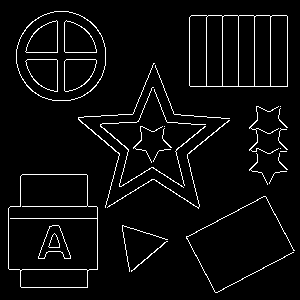
\includegraphics[width=.45\textwidth]{../examples/original/original-canny.png}\quad
				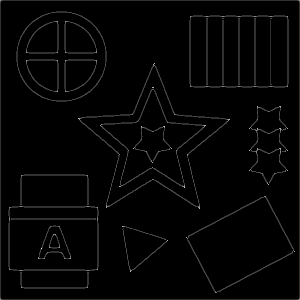
\includegraphics[width=.45\textwidth]{../examples/original/test_nonmax_supp.png}
				\caption{Links: Canny, Rechts: SUSAN.}
				\label{fig:canny_no_corners}
			\end{figure}

		\section{Heuristik}\label{sec:heuristic}
			 	Durch die folgende Heuristik aus \cite{SUSAN} soll dargestellt werden, wie das Prinzip des SUSAN-Kantendetektors funktioniert. Die Heuristik ist nicht als Beweis zu verstehen, da für diese Heuristik Annahmen getroffen werden, die nicht auf Digitalbilder zutreffen.

			 	Angenommen wir haben ein eindimensionales Bild. Unser Ziel ist es, genau die Stellen zu markieren, die den größten Grauwertunterschied zu ihrer Nachbarschaft haben. Das klassische Werkzeug der Analysis, um genau diese Stellen zu identifizieren, ist die Ableitung. Leiten wir eine zweimal differenzierbare, stetige Funktion $I$ zweimal ab, so erhalten wir eine Funktion $I''$, dessen Nullstellen die Stellen des größten Unterschieds in $I$ repräsentieren.

			 	So eine Ableitung existiert allerdings nicht für Digitalbilder. Darum nehmen wir zunächst an, dass unser Bild eine solche Funktion $I: [0, B-1]_\mathbb{R} \to [0,255]_\mathbb{R}$ ist. Implizit wird im Folgenden die Annahme getroffen, dass $I$ eine bijektive Funktion ist. Das ist im Allgemeinen zwar nicht der Fall, allerdings liegt uns bei der digitalen Verarbeitung von Bildern im Gegensatz zur eindimensionalen Analysis immer beides vor: Die Position und die Intensität eines Pixels lassen sich hier durch geschicktes Speichern aufeinander zurückführen.

			 	\begin{figure}[H]
			 		\centering
			 		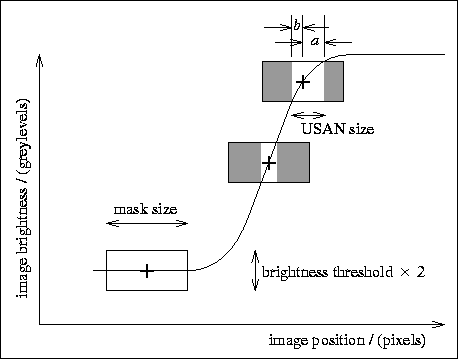
\includegraphics[width=.7\textwidth]{assets/susan-graph.png}
			 		\caption{Das Bild $I$ (Bild entnommen aus \cite{SUSAN}). Das Kreuz steht für den Nukleus der USAN und die Kästen für die Maske.}
			 		\label{fig:susan-graph}
			 	\end{figure}

				Der SUSAN-Kantendetektor beruht auf folgendem Prinzip: Für einen Schwellenwert $t$ gibt es, abhängig von der spezifischen Stelle im Bild $x_0$, eine obere Grenze $x_0+a(x_0)$ und eine untere Grenze $x_0-b(x_0)$ der USAN. In der Abbildung \ref{fig:susan-graph} ist an drei verschiedenen Stellen dargestellt, wie das Fenster für verschiedene $x_0$ variieren kann. Dies ist in Abbildung \ref{fig:susan-graph} für $x_0$ am mittleren Kreuz der Fall.
				Dann gilt an den Grenzen:
				\begin{align*}
					I(x_0 + a(x_0)) &= I(x_0) + t \\
					I(x_0 - b(x_0)) &= I(x_0) - t.
				\end{align*}
				Hier gehen wir von der Darstellung in Abbildung \ref{fig:susan-graph} aus. Falls die Intensitätsfunktion $I$ fallend ist, sind die Formeln entsprechend zu ändern.
				Das Prinzip des SUSAN-Kantendetektors lässt sich folgendermaßen formulieren: An genau den Stellen, an denen $n(x_0) := a(x_0) + b(x_0)$ ein Minimum hat, das heißt wenn die Fensterbreite am kleinsten ist, ist die Antwort $A(x_0) > 0$. Wir erhalten unter der Annahme, dass $n$ an $x_0$ ein lokales Minimum erreicht:
				$$ n'(x_0) = a'(x_0) + b'(x_0) = 0. $$
				Die obigen Gleichungen können wir nach $a$ und $b$ umstellen. So erhalten wir
				\begin{align*}
					a(x_0) = x(I(x_0) + t) - x_0, \\
					b(x_0) = x_0 - x(I(x_0) - t),
				\end{align*}
				wobei $x$ die Umkehrfunktion von $I$ ist.
				Damit ist $n(x_0) = x(I(x_0) + t) - x(I(x_0) - t)$ und daraus folgt
				$$ n'(x_0) = x'(I(x_0) + t) \cdot I'(x_0) - x'(I(x_0) - t) \cdot I'(x_0) = 0,$$
				anders formuliert
				$$ x'(I(x_0) + t) \cdot I'(x_0) = x'(I(x_0) - t) \cdot I'(x_0). $$
				Damit gilt
				$$
					x'(I(x_0) + t) = x'(I(x_0) - t) \quad \iff \quad x'(I(x_0 + a(x_0))) = x'(I(x_0 - b(x_0))),
				$$
				falls $I'(x_0) \neq 0$, das heißt falls die Bildfunktion $I$ nicht konstant ist.
	 			Aus der Inversenregel der Differenzialrechnung erhalten wir
	 			\begin{align*}
	 				x'(I(x_0 + a(x_0))) &= \frac{1}{I'(x_0 + a(x_0))},\\
	 				x'(I(x_0 - b(x_0))) &= \frac{1}{I'(x_0 - b(x_0))},
	 			\end{align*}
	 			und dadurch
	 			$$ I'(x_0 + a(x_0)) = I'(x_0 - b(x_0)), $$
	 			falls $I'(x_0 + a(x_0)) \neq 0$.
	 			Folglich ist die Approximation der zweiten Ableitung
	 			$$I''(x_0) \approx \frac{I'(x_0 + a(x_0)) - I'(x_0 - b(x_0))}{a(x_0) + b(x_0)} = 0.$$
	 			Also ist die Antwort des SUSAN-Kantendetektors in $x_0$ maximal, wenn die zweite Ableitung der Bildfunktion $I''(x_0) = 0$ ist. Tatsächlich verwendet der SUSAN-Kantendetektor allerdings keine Ableitungen, sondern diskrete Werte. Der SUSAN-Algorithmus bestimmt lediglich die Anzahl der ähnlichen Pixel in einer Umgebung.

				\begin{figure}[H]
					\begin{center}
						\begin{tikzpicture}[fill=orange]
							\matrix(m)[matrix of nodes, nodes={draw, minimum size = 0.5cm}, nodes in empty cells, column sep=-\pgflinewidth,row sep=-\pgflinewidth]{
										&|[fill]|	&|[fill]|	&|[fill=yellow]|	&|[fill]|	&|[fill]|	&	\\
							};
						\end{tikzpicture}
						\caption{Filtermaske im 1D-Bild. Der Nukleus ist gelb markiert. Die orangenen Pixel liegen innerhalb der Maske. Die weißen Pixel liegen außerhalb der Maske.}
						\label{fig:def_maske_1d}
					\end{center}
				\end{figure}

	 			In einem eindimensionalen Digitalbild $P: [0,B-1]_\mathbb{Z} \to [0,255]_\mathbb{Z}$ identifizeren wir durch eine Maske wie zum Beispiel in Abbildung \ref{fig:def_maske_1d} die USAN der einzelnen Pixel, wie auch schon im Algorithmus in \ref{sec:thealgorithm}. Dabei stellen wir für jede USAN fest, wie viele Pixel $r$ ähnlich zu dem Nukleus $r_0$ in der Mitte der Maske sind. Wir erinnern uns an die Definitionen aus dem Algorithmus
				$$
				A(r_0) = \text{max}\{0, g - n(r_0)\},\;
				n(r_0) = \sum_r c_t(r, r_0),\;
				c_t(r, r_0) =
					\begin{cases}
						1 	& \text{falls } |I(r) - I(r_0)| \leq t, 	\\
						0 	& \text{sonst.}
					\end{cases}
				$$

				Anhand eines Beispielbildes wird nun vorgeführt, wie der SUSAN-Kantendetektor eine Kante identifiziert.
				\begin{figure}[H]
					\begin{center}
						$\cdots$
						\begin{tikzpicture}[fill=black, text=white]
							\matrix(m)[matrix of nodes, nodes={draw, minimum size = .9cm}, column sep=-\pgflinewidth,row sep=-\pgflinewidth]{
								|[text=black, fill=white]|\phantom{H}	&|[text=black, fill=white]|\phantom{H}	&|[text=black, fill=white]|A	&|[text=black, fill=white]|B	&|[text=black, fill=white]|C	&|[fill]|D	&|[fill]|E	&|[fill]|F	 &|[fill]|\phantom{H} 	&|[fill]|\phantom{H} \\
							};
						\end{tikzpicture}
						$\cdots$
						\caption{Die weißen Pixel haben den Grauwert $255$, die schwarzen Pixel den Grauwert $0$.}
						\label{fig:1d-heur}
					\end{center}
				\end{figure}
				Wir stellen fest, dass die mit A-F markierten Pixel verschiedene Anzahlen an ähnlichen Nachbarn in ihrer Maske haben.
				\begin{align*}
					n(A) = 4,\quad n(B) = 3,\quad n(C) = 2,\\
					n(D) = 2,\quad n(E) = 3,\quad n(F) = 4.\\
				\end{align*}
				Entsprechend finden wir eine Antwort mit $g = 4$ wie in Abbildung \ref{fig:1d-ans}.
				\begin{figure}[H]
					\begin{center}
						$\cdots$
						\begin{tikzpicture}[fill=black, text=white]
							\matrix(m)[matrix of nodes, nodes={draw, minimum size = .9cm}, column sep=-\pgflinewidth,row sep=-\pgflinewidth]{
								&|[fill]|0	&|[fill]|1	&|[fill]|2	&|[fill]|2 &|[fill]|1 &|[fill]|0\\
							};
						\end{tikzpicture}
						$\cdots$
						$$\downarrow \cdot \frac{255}{\text{max}\{A(r)\}} \downarrow$$
						$\cdots$
						\begin{tikzpicture}[fill=black, text=white]
							\matrix(m)[matrix of nodes, nodes={draw, minimum size = .9cm}, column sep=-\pgflinewidth,row sep=-\pgflinewidth]{
								|[fill=white!0!black]|0	&|[fill=white!50!black]|128	&|[fill=white!100!black, text=black]|255	&|[fill=white!100!black, text=black]|255	&|[fill=white!50!black]|128	&|[fill=white!0!black]|0	\\
							};
						\end{tikzpicture}
						$\cdots$
						$$\downarrow \text{Non-Max-Supp.} \downarrow$$
						$\cdots$
						\begin{tikzpicture}[fill=black, text=white]
							\matrix(m)[matrix of nodes, nodes={draw, minimum size = .9cm}, column sep=-\pgflinewidth,row sep=-\pgflinewidth]{
								|[fill=white!0!black]|0	&|[fill=white!0!black]|0	&|[fill=white!100!black, text=black]|255	&|[fill=white!100!black, text=black]|255	&|[fill=white!0!black]|0	&|[fill=white!0!black]|0	\\ 
							};
						\end{tikzpicture}
						$\cdots$
						\caption{Antwort}
						\label{fig:1d-ans}
					\end{center}
				\end{figure}
				Durch das SUSAN-Prinzip und die Non-Maximum-Suppression konnten wir die Kante ohne Ableitung bestimmen.

		\chapter{Diskussion}
			Der SUSAN-Kantendetektor findet Kanten auf digitalen Bildern einfach, schnell und pixelgenau, wie wir an mehreren Beispielen erkennen konnten. Im Gegensatz zum Kantendetektor von Canny eignet sich SUSAN auch zur Identifikation von Ecken.

			Meine persönliche Implementation könnte trotz Einbindung von \texttt{multiprocessing} noch schneller sein, dazu würden sich einerseits GPU-gestützte Methoden sowie auch eine Implementation in einer weniger dynamischen Sprache wie zum Beispiel \texttt{C++} anbieten (siehe \cite{pyslow}). Die Implementation in Python 3 bietet aber den großen Vorteil der Modifizierbarkeit, was einerseits die Fehlersuche und andererseits das Experimentieren mit verschiedenen Maskenträgern und Randbedingungen erleichtert. Im Sinne einer Bachelorarbeit, welche nicht notwendigerweise einen industriellen Nutzen tragen muss, bewerte ich die Wahl der Sprache aus diesem Grund als gelungen.

			Der Kantendetektor von Canny hingegen ist durch die Vektorisierbarkeit der Faltung in Python 3 mit kürzeren Laufzeiten zu realisieren. Dadurch fielen nämlich zahlreiche \texttt{for}-Schleifen weg, welche aufgrund vorher genannter dynamischer Natur von Python 3 der Flaschenhals meiner Implementation des SUSAN-Kantendetektors sind.

			Der Kantendetektor von Canny basiert auf dem Prinzip der Diskretisierung der Ableitung, wohingegen der SUSAN-Kantedetektor auf einem kombinatorischen Prinzip basiert, welches in \cite{SUSAN} nur über eine Analogie mit der eindimensionalen Analysis erklärt wurde, ähnlich, wie in Kapitel \ref{sec:heuristic}. Das Fehlen der mathematischen Gründlichkeit für eine Herleitung des SUSAN-Kantendetektors steht einer vergleichsweise einfachen Strategie des Zählens der ähnlichen Nachbarn gegenüber.
\pagebreak
\pagestyle{plain}


\begin{thebibliography}{56}
\bibitem{SUSAN}
	Stephen M. Smith, J. Michael Brady,\\
	\textit{SUSAN - A New Approach to Low Level Image Processing},\\
	International Journal of Computer Vision 23(1), 45-78,\\
	1997

\bibitem{thinout}
	Stephen M. Smith,\\
	\textit{Edge Thinning Used in the SUSAN Edge Detector},\\
	Technical Report TR95SMS5,\\
	1995

\bibitem{gaussianblur}
	Robert Fisher, Simon Perkins, Ashley Walker, Erik Wolfart,\\
	\textit{Gaussian Smoothing},\\
	The Hypermedia Image Processing Reference 2,\\
	2004
	
\bibitem{pillow}
	Pillow: the friendly PIL fork, \\
	\texttt{https://python-pillow.org/}

\bibitem{numpy}
	NumPy,\\
	\texttt{https://numpy.org/}

\bibitem{multiprocessing}
	multiprocessing - Process-based parallelism, \\
	\texttt{https://docs.python.org/3/library/multiprocessing.html}

\bibitem{pyslow}
	Jake VanderPlas,\\
	\textit{Why Python is Slow: Looking Under the Hood},\\
	\texttt{https://jakevdp.github.io/blog/2014/05/09/why-python-is-slow/},\\
	2014

\bibitem{pyparallel}
	Markus Konrad,\\
	\textit{Vectorization and parallelization in Python with NumPy and Pandas},\\
	\texttt{https://datascience.blog.wzb.eu/2018/02/02/\\
	vectorization-and-parallelization-in-python-with-numpy-and-pandas/},\\
	2018

\bibitem{canny}
	John Canny,\\
	\emph{Finding lines and edges in images},\\
	Technical Report TM-720,\\
	Artificial Intelligence Laboratory, Massachusetts Institute of Technology,\\
	1983

\bibitem{mysoftware}
	Julian Lüken,\\
	Implementation des SUSAN Kantendetektors in Python 3,\\
	\texttt{https://gitlab.gwdg.de/julian.lueken/susan/},\\
	2019

\end{thebibliography}
\pagebreak


\pagestyle{headings}
\appendix
\chapter{Quellcode}
\lstinputlisting[basicstyle=\tiny\ttfamily, frame=single,label=Susan.py, breaklines=true, postbreak=\mbox{\textcolor{red}{$\hookrightarrow$}\space}]{../python/Susan.py}

% zu den quellen:
%
% blabla überschreitet den rahmen dieser arbeit (weiterführende literatur)
% beobachtungen zum vergleich
% grundlagen
% paper auf denen meine arbeit basiert xD

\end{document}
